%version of 04-10-20

\chapter{Summations:
Complex Operations from Simple Components}
\label{ch:Summation}


\section{Introducing the Many Facets of Summation}
\label{sec:intro}

The operation of {\it summation}---adding up aggregations of numbers---is of fundamental importance in the world of digital computing.  While we humans are able to deal handily with abstractions such as ``smoothness'' and ``continuity'', we must employ sophisticated {\em discretizations} of these concepts in order to enlist the aid of digital computers in dealing with such abstractions.  Summations provide a very useful discretization of {\em continuous} (or,
``smooth'') phenomena that are typically dealt with with the aid of the (differential and integral) calculus.

\medskip

This chapter is dedicated to exploring how to employ summations as a computational tool.  We deal throughout with {\it series}, {\it i.e.}, (possibly infinite) sequences of numbers
\[ a_1, a_2, a_3, \ldots \]
whose sum
\begin{equation}
\label{eq:abstract-sum}
a_1 + a_2 + a_3 + \cdots
\end{equation}
is the target of interest.

\medskip

\noindent \fbox{
\begin{minipage}{0.96\textwidth}
{\bf Explanatory note \#1}.

Of course, when we deal with {\em infinite} series, wherein there are infinitely many numbers $a_i$, we must address the question of whether the sum (\ref{eq:abstract-sum}) exists as a finite number.  For some infinite series the sum {\em does} exist:  We note, for example, the well-known sum
\begin{equation}
\label{eq:sample-sum-2^(-k)}
 1 \ + \ \frac{1}{2} \ + \ \frac{1}{4} \ + \ \frac{1}{8} \ +
\ \frac{1}{16} \ + \ \cdots \ + \ \frac{1}{2^k}  \ +
\ \frac{1}{2^{k+1}} \ + \ \cdots \ = \ 2 
\end{equation}
(We shall encounter this summation in several guises during our journey through this text.)  Infinite series such as (\ref{eq:sample-sum-2^(-k)}) are said to {\em converge}.
\index{infinite series!convergent}
\end{minipage}
}

\noindent \fbox{
\begin{minipage}{0.96\textwidth}
{\bf Explanatory note \#2}.

But sometimes an infinite series does {\em not} have a finite sum.  This is true, for instance, with the well-known {\it harmonic} series \index{harmonic series}
\begin{equation}
\label{eq:sample-sum-harmonic}
1 \ + \ \frac{1}{2} \ + \ \frac{1}{3} \ + \ \frac{1}{4} \ +
\ \frac{1}{5} \ + \ \cdots \ + \ \frac{1}{k} \ + \ \frac{1}{k+1} \ +
\ \cdots
\end{equation}
As more and more terms are added to this summation, the accumulated sum eventually exceeds every number.  Such an infinite series is said to {\em diverge}.
\index{infinite series!divergent}

\smallskip

Summations such as (\ref{eq:sample-sum-harmonic}) diverge because their initial partial sums---i.e., the sequence $1$, $1 + \frac{1}{2}$, $1 + \frac{1}{2} + \frac{1}{3}$, \ldots, for (\ref{eq:sample-sum-harmonic})--grow without bound.  There are other infinite series whose behavior is harder to describe.  One such example is the series
\[ 1 \ - \ 1 \ + \ 1 \ - \cdots + \ 1 \ - \ 1 \ + - \cdots \] 
which we discuss briefly in the exercises of this chapter and in Chapter~\ref{ch:infinity}.
\end{minipage}
}

\medskip

Sums such as (\ref{eq:sample-sum-2^(-k)}) and (\ref{eq:sample-sum-harmonic}) illustrate some of the complexity of dealing with infinite entities.  Most obviously, as we have just remarked, when the summations are infinite, some of them have finite sums while others do not.  Even more subtle, the series that {\em do} have (finite) sums illustrate the unintuitive fact that sometimes finite objects or entities---such as the integer $2$ in equation (\ref{eq:sample-sum-2^(-k)})---have infinite ``names'':  In this example, the series is an infinite ``name" of integer $2$.  Lots to think about!

\bigskip

\noindent \fbox{
\begin{minipage}{0.96\textwidth}
{\bf Enrichment note} (part 1).

The conceptual dissonance of dealing with {\em infinite objects} that have {\em finite values}---as exemplified by the series (\ref{eq:sample-sum-2^(-k)})---has been recognized in various forms for more than $25$ centuries.  Several charming and familiar examples appear in the paradoxes attributed to Zeno of Elea. \index{Zeno of Elea} \index{Zeno!Zeno's paradox} 

\smallskip

In his {\it Paradox of Achilles and the Tortoise}, for instance, Zeno appears at first glance to prove that all motion is illusory!  In this story, the slow-of-foot Tortoise (T) tries to convince the speedy Achilles (A) of the futility of trying to win any race in which A gives T even the most minute head start.  As long as T is ahead of A, argues T, every time A traverses half the distance between the competitors, T will respond by moving a bit further ahead.  Thereby, T will always be a positive distance ahead of A, so that A can {\em never} catch T.

\smallskip

A similar ``argument'' demonstrates that an arrow shot at you by an adversary can never reach you, as long as you continually move away from the archer.  {\em DO NOT TRY THIS AT HOME!}
\end{minipage} }

\medskip

\noindent \fbox{
\begin{minipage}{0.96\textwidth}
{\bf Enrichment note} (part 2).

\index{infinitesimals} \index{Newton, Isaac} \index{Leibniz (Leibnitz), Gottfried Wilhelm}
The notion of {\em infinitesimals},  as invented by Isaac Newton and Gottfried Wilhelm Leibniz, explains the fallacy of assertions such as the Tortoise's.  This notion, which plays a huge role in modern mathematics, underlying such foundational concepts as {\em limits} and {\em continuity} (of functions), was not well understood until just a few hundred years ago.
 \index{limits}  \index{continuity (of functions)}

\medskip

The general topic of the convergence or divergence of infinite series is beyond the scope of this text, but we shall observe several examples of each concept throughout this chapter.  It is a fascinating subject for further study.
\end{minipage}
}

\bigskip

Toward the end of guiding the reader through the forest of abstractions and operations and techniques associated with summations, we categorize the targets of our discussions in three ways.
\begin{enumerate}
\item
We study a number of {\it fundamental summations} which have intrinsic interest.

\smallskip

Examples of this topic category include {\it arithmetic summations}, {\it geometric summations}, and {\it mathematically ``smooth'' summations}, including sums of positive and negative powers of integers.  Here is a sampler of six summations that appear later in this chapter.
\[
\begin{array}{lclcl}
1.  & &
1 \ + \ 2 \ + \ 3 \ + \ 4 \ + \ 5 \ + & \cdots & + \ k  \ + \ (k+1) \ + \ \cdots \ + \ n \\
2. & &
1 \ + \ 2 \ + \ 4 \ + \ 8 \ + \ 16 \ + & \cdots & + \ 2^k  \ + \ 2^{k+1} \ + \ \cdots \ + \ 2^n \\
3. & &
1 \ + \ 4 \ + \ 9 \ + \ 16 \ + \ 25 \ + & \cdots & + \ k^2  \ + \ (k+1)^2 \ + \ \cdots \ + \ n^2 \\
\smallskip
4. & &
1 \ + \ \frac{1}{2} \ + \ \frac{1}{4} \ + \ \frac{1}{16} \ + \ \frac{1}{32} \ + & \cdots & + \ \frac{1}{2^k}  \ + \ \frac{1}{2^{k+1}} \ + \ \cdots \\
\smallskip
5. & &
1 \ + \ \frac{1}{2} \ + \ \frac{1}{3} \ + \ \frac{1}{4} \ + \ \frac{1}{5} \ + & \cdots & + \ \frac{1}{k}  \ + \ \frac{1}{k+1} \ + \ \cdots \\
\smallskip
6. & &
1 \ + \ \frac{1}{4} \ + \ \frac{1}{9} \ + \ \frac{1}{16} \ + \ \frac{1}{25} \ + & \cdots & + \ \frac{1}{k^2}  \ + \ \frac{1}{(k+1)^2} \ + \ \cdots
\end{array}
\]

\item
We study a variety of {\it fundamental techniques} for evaluating summations.

\smallskip

We include specialized techniques that work for specific classes of summations, as well as more general techniques that work in a broad range of situations.

\smallskip

Examples of such techniques include, e.g.: estimating summations by integrating functions related to the summation; grouping/replication of terms within a summation; verifying ``guessed'' sums via induction.

\item
We study a variety of {\it fundamental representations} of the elements being summed.  We observe that being able to study the same phenomenon in a variety of seemingly unrelated ways often gives one unexpected mathematical understanding of, and operational control over, the phenomenon.

\smallskip

Examples of such representations include, among others, representations of numbers by: numerals in a positional number system; slices of pie; tokens arranged in stylized ways; basic geometrical structures, including the unit-width rectangles of so-called Riemann sums.
\end{enumerate}

\medskip

\noindent
{\em In conclusion, we treat each topic in multiple ways, as long as each new way supplies new intuition and teaches a new lesson.}

\bigskip

%%%%%%%%%%%%%%%%%%%%%%%%%%%%%%%%%%%%%%%%%%%%%%%%


\ignore{********\Denis Again, as I said before, I am not really convinced by this example.
Keeping the same sum, I prefer the story of Sissa, telling an old legende:
where wheat or rice is placed upon each square of the chess board in the following way:
put one grain on the first square, and then, double this number on each of the subsequent squares,
$2$ in the second case, $4$ in the third and so on.
**********}

\ignore{\Denis add cross reference for computing the sum of powers of 2 in DOINGMATHS}

\index{Sissa ibn Dahir, legend of} 
To illustrate the power of summation methodology, consider the following modernized version of the {\it legend of Sissa ibn Dahir}.  Sissa, goes the legend, has invented a marvelous game that is played on a chessboard, i.e., an $8 \times 8$ array of unit-size squares.  An entrepreneur proposes to buy the rights of this marvelous game from Sissa.  The entrepreneur offers Sissa a one-time payment of {\em one million million (i.e., $10^{12} = 1,000,000,000,000$) euros} in return for all rights to the new game\footnote{The original legend was about grains of rice, this is what is called {inflation}...}.  As a counter-offer, Sissa asked the entrepreneur instead for all of the money amassed in the following way.  Sissa requested that the entrepreneur proceed row by row along a chessboard, placing money in the board's squares, according to the following regimen.  The entrepreneur should place $1$ euro in the first square, $2$ euros in the second square, $4 \ (= 2 \times 2)$ euros in the third square, $8 \ (= 4 \times 2)$ euros in the
fourth square, and so on, doubling the number of euros at each step of the procedure---so the last square would contain $2^{63}$ euros. Fig.~\ref{fig:Sissa} illustrates the growth of the pile of euros during first few steps of the procedure.
\begin{figure}[ht]
\begin{center}
       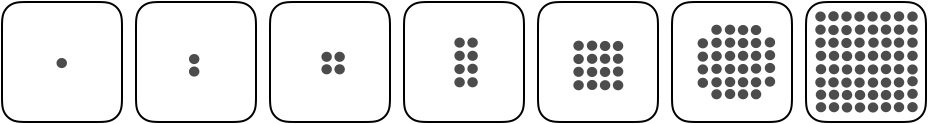
\includegraphics[scale=0.3]{FiguresMaths/chess}
\caption{The money in the first seven squares of the chessboard based on Sissa's counteroffer.}
       \label{fig:Sissa}
\end{center}
\end{figure}

\medskip

\noindent
{\em Has Sissa made a good bargain?}

\medskip

\noindent
By the end of this chapter, you will be able to determine in minutes that under the procedure that amasses money on the chessboard, Sissa would receive $2^{64} -1$ euros---which is more than $10^{20}$ euros!  Sissa would, therefore, amass {\em much} more money via his counteroffer than the mere $10^{12}$ euros that the entrepreneur offered!
%{\Denis I think the previous value is -1 and not -2}

\noindent
{\em A good bargain, indeed!}

%%%%%%%%%%%%%%%%%%%%%%%%%%%%%%%%%%%%%%%%%%%%%%%%%%%%


\section{Summing Structured Series}
\label{sec:structured-series}

\subsection{Arithmetic Summations and Series}
\label{sec:arithmetic-series}

\subsubsection{General development}

We define {\it arithmetic sequences} and learn how to calculate their sums, {\it arithmetic series}.
\index{arithmetic sequence} \index{arithmetic series}
\index{arithmetic sequence!period} \index{arithmetic series!period}
\begin{equation}
\label{eq:arith-seq}
\begin{array}{l}
\mbox{An $n$-term {\em arithmetic sequence}:} \\
\hspace*{.25in}a, \ a+b, \ a+2b, \ a+3b, \ \ldots, a+(n-1)b \\
  \\
\mbox{The corresponding {\em arithmetic series}:} \\
\hspace*{.25in}a + (a+b) + (a+2b) + (a+3b) + \cdots + (a+(n-1)b) \\
\hspace*{.25in} = \
an + b \cdot (1 + 2 + \cdots + n-1)
\end{array}
\end{equation}
The common inter-element difference $b$ in the sequence and the series in (\ref{eq:arith-seq}) is the {\it period} of the sequence and the series.
 
The message from the factorization of the arithmetic series in (\ref{eq:arith-seq}) is that we can calculate the sum of the series by determining the sum of the first $n-1$ positive integers.  In the next subsection, we use this fact as an opportunity to introduce important notation.

\subsubsection{Example \#1: Summing the first $n$ integers}
\label{sec:special-arithmetic-sums}

\index{closed-form expression}
Our first goal in this section is to sum the first $n$ positive integers:
\[ 1 \ + \ 2 \ + \cdots + \ n \]
that is, to find a {\it closed-form expression} for the sum.  In somewhat informal terms, we say that an expression of the type
\begin{equation}
\label{eq:sigma-summation}
f(n) \ \eqdef \ \sum_{i=1}^n \ i
\end{equation}
is in {\it closed form} if it provides a prescription for evaluating the sum using a {\em fixed-length} sequence of arithmetic operations (e.g., addition/subtraction, multiplication/division, exponentiation/taking logarithms).  The notion ``closed form" contrasts with the recipe implicit in the notation (\ref{eq:sigma-summation}), which takes $n-1$ additions to evaluate---because its length depends on input $n$, the indicated computation does not have {\em fixed} length. 

\index{$\Delta_n$: sum of the first $n$ integers}
The sum $f(n)$ of the special summation  (\ref{eq:sigma-summation}) is commonly denoted $\Delta_n$.  Within this chapter, we usually prefer the notation $S_1(n)$ for this sum, because it
exposes this summation as one instance of a related family of such summations that will occupy us through this chapter; we denote the sums of these summations by the notation $S_c(n)$ for various values of parameter $c$.

\smallskip

The remainder of this section develops multiple ways to derive the following {\em closed-form} expression for $\Delta_n = S_1(n)$.

\begin{prop}
\label{thm:sum-first-integers-Gauss}
\index{sum of first $n$ integers}
For all $n \in \N$,
\begin{equation}
\label{eq:sum-1-to-n}
S_1(n) \ = \ \sum_{i=1}^n \ i \  \ = \  \frac{1}{2} n (n+1) 
\end{equation}
\end{prop}
\index{Sum of the first $n$ integers: $\Delta_n = S_1(n)$}

%{\Denis I removed the last equality with n+1 choose 2 since this
%combinatorial proof is presented later...}

\index{Sum of the first $n$ integers: $\Delta_n = S_1(n)$!a {\bf textual} derivation}
\index{Gauss, Karl Friedrich} \index{Gauss, Karl Friedrich!summation ``trick''}
\index{sum of first $n$ integers!a textual reckoning}
\begin{proof}
{\bf A textual proof.}
We begin with a {\em constructive, textual} proof\footnote{The proof is {\em constructive:} it actually derives an explicit answer.  This contrasts with, say, the inductive validation of the sum $S_1(n)$ in Section~\ref{sec:positive-integer-power}.C, which just verifies a ``guessed'' answer.}~of summation (\ref{eq:sum-1-to-n}) which employs an approach that was, famously,  used in a school exercise by the eminent German mathematician Karl Friedrich Gauss---as a pre-teenager.  This approach proceeds in two steps.
\begin{equation}
\label{eq:arith-series}
\begin{array}{llccccccccc}
\mbox{Write $S_1(n)$ ``forwards'':} &
\hspace*{.2in}\sum_{i=1}^n \ i \ = & 1 & + & 2   & + & \cdots & + & (n-1) & + & n \\
 & & & & & & & & & &  \\
\mbox{Write $S_1(n)$ ``in reverse'':} &
\hspace*{.2in}\sum_{i=n}^1 \ i \ = & n & + & (n-1) & + & \cdots & + & 2   & + & 1
\end{array}
\end{equation}
Now add the two representations of $S_1(n)$ in (\ref{eq:arith-series})
{\em column by column}.  Because each of the $n$ column-sums equals $n+1$, we find that $2 S_1(n) = n(n+1)$, which we easily rewrite in the form (\ref{eq:sum-1-to-n})---after we multiply both sides of the equation by $2$.
\end{proof}

\medskip
\noindent \fbox{
\begin{minipage}{0.96\textwidth}
{\bf Explanatory note}.

Let us step back from the specific result in Proposition~\ref{thm:sum-first-integers-Gauss} and concentrate on the textual proof.  What Gauss noticed about the problem of computing $S_1(n)$ is that when the sum is doubly written as in (\ref{eq:arith-series}), the column-sums are all the same.  This phenomenon of finding {\em invariants} is a ``pattern'' of the form referred to in Chapter~\ref{ch:doingmath} as we discussed how to ``do mathematics''.  We observe how the pattern can be exploited to determine the sum of any arithmetic series.  {\em What seemed to be a ``trick'' turns out to be an insightful instance of pattern-matching!}  We soon see how to employ the pattern for other, related, ends.
\end{minipage}
}

\bigskip

Not everyone thinks the same way---even within the context of mathematics.  It is, therefore, very important for the reader to recognize that even the simplest mathematical facts can be proved and analyzed in a broad variety of ways.  We illustrate this assertion by developing several more proofs of Proposition~\ref{thm:sum-first-integers-Gauss}.

\index{Sum of the first $n$ integers: $\Delta_n = S_1(n)$!a {\bf ``pictorial'', graphic} derivation}
\index{unit-side square}
\begin{proof}
{\bf A ``pictorial'', graphical proof.}
Now we shall look at the problem of summing $S_1(n)$ by estimating the area of a simple (in the \textit{good sense} of the word) surface.  In this worldview, integers are represented by concatenating {\it unit-side} (i.e., $1 \times 1$ {\it squares}), as in Fig.~\ref{fig:sumIntegersGeo1}.

\smallskip

Our summation process proceeds in the three steps illustrated in Figs.~\ref{fig:sumIntegersGeo1}-\ref{fig:sumIntegersGeo2}.
\begin{enumerate}
\item
We begin, in Fig.~\ref{fig:sumIntegersGeo1}, by depicting the problem of calculating $S_1(n)$ as the problem of determining the area of a surface built from unit-side squares.
\begin{figure}[htb]
\begin{center}
       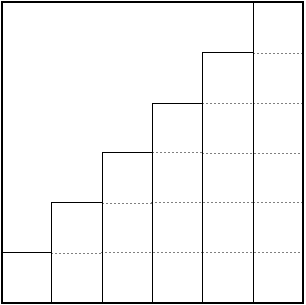
\includegraphics[scale=0.33]{FiguresMaths/SumIntegersGeometricBasis}
\caption{Representing the first $n$ integers using unit squares; $n=6$ in this example.}
       \label{fig:sumIntegersGeo1}
\end{center}
\end{figure}

\item
Next, we illustrate in Fig.~\ref{fig:sumIntegersGeo2}(Left) that the area of the (light grey) lower-right triangle of the $n \times n$ square is one-half the area of the entire $n \times n$ square.
\begin{figure}[htb]
\begin{center}
       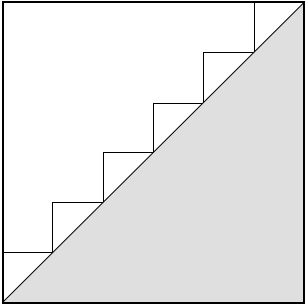
\includegraphics[scale=0.33]{FiguresMaths/SumIntegersGeometricIntermediate}
       \hspace*{.25in}
        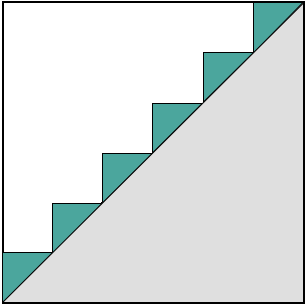
\includegraphics[scale=0.33]{FiguresMaths/SumIntegersGeometricFinal}
\end{center}
\caption{(Left) The area of the lower-right triangle (light grey) is one-half that of the entire $n \times n$ square.  (Right) The area of the (dark) triangles upon the upper diagonal of the $n \times n$ square is ${1 \over2} n$.}
       \label{fig:sumIntegersGeo2}
\end{figure}

\item
Finally, we indicate in Fig.~\ref{fig:sumIntegersGeo2}(Right) that the cumulative area of the small (dark grey) triangles which sit on the upper diagonal of the $n \times n$ square is ${1 \over 2} n$.  This reckoning notes that there are $n$ triangles, each of area equal to one-half the area of a unit-side square.
\ignore{**************
\begin{figure}[htb]
\begin{center}
       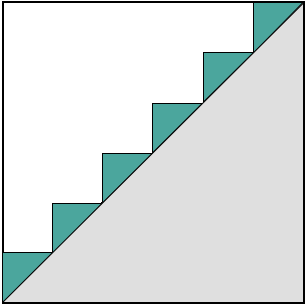
\includegraphics[scale=0.35]{FiguresMaths/SumIntegersGeometricFinal}
\caption{The area of the (dark) triangles sitting on the upper diagonal of the $n \times n$ square is $\frac{1}{2} n$.}
       \label{fig:sumIntegersGeo3}
\end{center}
\end{figure}
***************}
\end{enumerate}
We thereby reckon the area of the surface depicting $S_1(n)$ as

\begin{tabular}{l}
{\it One-half the area of the $n \times n$ square,
i.e., $\frac{1}{2} n^2$} \\
\hspace*{.15in} plus   \\
{\it $n$ times the area of one-half a unit-side square,
i.e., $\frac{1}{2} n$}
\end{tabular}

\smallskip

\noindent
This reasoning thus derives the value of $S_1(n)$.
\end{proof}

\medskip

We present one final, combinatorial, proof of Proposition~\ref{thm:sum-first-integers-Gauss}.

\index{Sum of the first $n$ integers: $\Delta_n = S_1(n)$!a {\bf combinatorial} derivation}
\begin{proof}
{\bf A combinatorial proof.}
The following argument is {\it combinatorial} in that it achieves its goal by {\em counting} instances of the first $n$ integers, laid out in a line.

\smallskip

Place (tokens that represent) the integers $0$ to $n$ along a line.  For each integer $i$, count how many integers $j > i$ lie to its right.  We see that in general, there is a {\it block} of $n-i$ integers that lie to the right of integer $i$.  In detail: the block of integers lying to the right of $i=0$ contains $n$ values of $j$; the block to the right of $i=1$ contains $n-1$ values of $j$, and so on, as suggested in Fig.~\ref{fig:rightward-instances}.
\begin{figure}[htb]
\[
\begin{array}{lcccccc}
\mbox{All integers $\leq 4$:} &
 & 0 & 1 & 2 & 3 & 4 \\
\mbox{integers to the right of $0$:} &
 &   & 1 & 2 & 3 & 4 \\
\mbox{integers to the right of $1$:} &
 &   &   & 2 & 3 & 4 \\
\mbox{integers to the right of $2$:} &
 &   &   &   & 3 & 4 \\
\mbox{integers to the right of $3$:} &
 &   &   &   &   & 4
\end{array}
\]
\caption{A two-dimensional (triangular) depiction of the right-lying integer-instances.}
\label{fig:rightward-instances}
\end{figure}

\smallskip

On the one hand, we see that the total number, $j$, of right-lying integers equals $n+(n-1)+ \cdots + 1 \ = \ S_1(n)$.

\smallskip

On the other hand, every instance of a right-lying integer can be identified uniquely by the pair of nonnegative integers, $i$ (the instance's block) and $j>i$ (the instance's position-within-block).
The total number of right-lying integer-instances corresponds to the number of ways one can select two objects (here, integers) from among $n+1$ objects.\footnote{We study such counting techniques in depth in Section~\ref{sec:counting}.}  This number is the {\it binomial coefficient }, whose definition we specialize from equation (\ref{eq:binom-coeff}) in Section~\ref{sec:binary-operators}.C:
\[
\Delta_n  \ = \  {{n+1} \choose 2}  \  \eqdef  \  \frac{1}{2} n(n+1)
\]
We have thus derived two distinct---but, of course, equal---expressions for $S_1(n)$.
\end{proof}

\medskip

\noindent \fbox{
\begin{minipage}{0.96\textwidth}
{\bf Explanatory note.}

We have now exposed the sums $\Delta_n$ as special binomial coefficients, namely, those whose ``bottom" parameter is $2$.  The many ways of viewing the underlying summation in terms of {\em triangles}---as in Figs.~\ref{fig:sumIntegersGeo1}--\ref{fig:rightward-instances}---have led to the naming of these special binomial coefficients as {\it triangular numbers}.
\index{triangular numbers}  \index{binomial coefficients!triangular numbers} 
\end{minipage}
}

\medskip

\noindent \fbox{
\begin{minipage}{0.96\textwidth}
{\bf Cultural note}.

Our combinatorial derivation of summation (\ref{eq:sum-1-to-n}) illustrates one of the most important roles of mathematical abstraction.  There is no obvious intuition to explain the relationship between the activity of summing $n$ consecutive integers and the activity of extracting two objects out of a set of $n$ objects.  Yet, our combinatorial derivation exposes an intimate connection between the two.
\end{minipage}
}

\bigskip

Now that we know---{\em and understand}---how to derive the value of $S_1(n)$, we can finally evaluate our original series in (\ref{eq:arith-seq}).  \index{arithmetic series:explicit sum}

\begin{prop}
\label{thm:sum-of-arithmetic-series}
The arithmetic series in (\ref{eq:arith-seq}) has the sum
\begin{equation}
\label{eq:sum-arithmetic-series}
a + (a+b) + (a+2b) + (a+3b) + \cdots + (a+(n-1)b) \ \ = \ \
an + b \cdot \Delta_n
\end{equation}
\end{prop}


\subsubsection{Example \#2: Squares as sums of odd integers}
\label{sec:sumOfOdds}

In this section, we build on Proposition~\ref{thm:sum-first-integers-Gauss} to craft multiple constructive proofs of the fact that each perfect square $n^2$ is the sum of the first $n$ odd integers, $1, 3, 5, \ldots, 2n-1$.  All of these proofs complement the ``guess-and-verify'' inductive
proof of this result in Section~\ref{sec:positive-integer-power}.C.

\begin{prop}
\label{thm:squares-odd-integers-Gauss}
\index{$n^2$ as sum of first $n$ odd integers}
For all $n \in \N^+$,
\begin{equation}
\label{eq:sum-of-odds}
\sum_{i=1}^n \ (2i-1)
 \ = \ 1 + 3 + 5 + \cdots + (2n-1) \ = \ n^2
\end{equation}
That, is, the $n$th perfect square is the sum of the first $n$ odd integers.
\end{prop}

Before we present our proofs of this result, we want to stress that the notation for odd integers in the summation within (\ref{eq:sum-of-odds}) is completely general: {\em Every positive odd integer can be written in the form $2i-1$ for some positive integer $i$.}

\bigskip

Our first two proofs of Proposition~\ref{thm:squares-odd-integers-Gauss} note that the result is a corollary of both Proposition~\ref{thm:sum-first-integers-Gauss} and Proposition~\ref{thm:sum-of-arithmetic-series}.

\medskip

\index{$n^2$ as sum of first $n$ odd integers!a proof using algebra}
\begin{proof}
{\bf A proof using algebra.}
By direct calculation, we find that
\begin{eqnarray*}
\sum_{i=1}^n \ \left( 2i-1 \right)
   & = & 2 \sum_{i=1}^n \ i \ \ - \ n \\
   & = & 2 \Delta_n \ \ - \ n \ \ \ \ \ \ \ \ \ \ \mbox{ (by
  Proposition~\ref{thm:sum-first-integers-Gauss})} \\
   & = & (n^2 + n) - n \\
   & = & n^2
\end{eqnarray*}
\end{proof}

\medskip

\index{$n^2$ as sum of first $n$ odd integers!a proof by calculation}
\begin{proof}
{\bf A proof by calculation.}
%
Because summation (\ref{eq:sum-of-odds}) is an arithmetic series with parameters $a=1$ and $b=2$, we know from Proposition~\ref{thm:sum-of-arithmetic-series} that the summation evaluates to
\[ (1 \cdot n) + 2 \Delta_{n-1} \ = \ n + n^2 -n \ = \ n^2 \]
\end{proof}

\ignore{***\Denis According to the
  expression of Proposition~\ref{thm:sum-of-arithmetic-series}, the
  sum is equal to $1.n + 2 \Delta_{n-1} = n + n^2 -n = n^2$.  Let us
  detail several alternative proofs.***}

\medskip

Our next proof builds on the stratagem of {\em finding invariants} that we exploited in the textual proof of Proposition~\ref{thm:sum-first-integers-Gauss}.

\index{$n^2$ as sum of first $n$ odd integers!a textual proof}
\begin{proof}
{\bf A textual proof.}
We adapt Gauss's ``trick'' to this summation ; i.e., we write the current summation both forwards and backwards, and then add the two summations term by term.  Let us denote the target summation $\sum_{k=1}^n \ (2k-1)$ by $S(n)$.  We record $S(n)$ both forwards and backwards:
\begin{equation}
\label{eq:add-odds}
\begin{array}{llccccccccc}
\mbox{``Forwards'':} &
S(n) \ = 
& 1 & + & 3 & + & \cdots & + & (2n-3) & + & (2n-1) \\
 & & & & & & & & & &  \\
\mbox{``Backwards'':} &
S(n) \ =
& (2n-1) & + & (2n-3) & + & \cdots & + & 3 & + & 1
\end{array}
\end{equation}
Now, we add these two representations of $S(n)$ {\em column by column}.  Because each of the $n$ column-sums equals $2n$, we find that
\begin{equation}
\label{eq:sum-of-odds-sum}
2 S(n) \ = \ 2 \sum_{i=1}^n \ (2i-1) \ = \ 2n^2
\end{equation}
We thus derive the sum (\ref{eq:sum-of-odds}) when we halve (i.e., divide by $2$) the three
equated quantities in equation (\ref{eq:sum-of-odds-sum}).
\end{proof}

\medskip

\index{$n^2$ as sum of first $n$ odd integers!a ``pictorial" proof}
\begin{proof}
{\bf A ``pictorial" proof.}
We now build up to a proof that is almost purely pictorial, with only a bit of reasoning turning the pictures into a narrative.  The only ``sophisticated'' knowledge this proof requires is that
\begin{equation}
\label{eq:(n+1)^2}
(n+1)^2 \ = \ n^2 \ + \ 2n \ + \ 1
\end{equation}
This well-known equation is verified by symbolically {\em squaring} expression $n+1$:
\[ (n+1) \times (n+1) \ \ = \ \ n \cdot (n+1) \ + \ (n+1) 
     \ \ = \ \ n^2 \ + \ n \ + \ n \ + \ 1
\]

\medskip

\noindent \fbox{
\begin{minipage}{0.96\textwidth}
{\bf Enrichment note}.

Equation (\ref{eq:(n+1)^2}) is the simplest instance of the {\em restricted Binomial Theorem}, which appears later in this chapter, as Theorem~\ref{thm:restricted-binomial-thm}.
\end{minipage}
}

\medskip

Our pictorial proof begins by representing the generic positive integer $n$ as a horizontal sequence of $n$ tokens, i.e., darkened circles.  The problem of summing the first $n$ odd integers then begins with a picture such as appears in Fig.~\ref{fig:sumOdds1}, for the illustrative case $n=5$.
\begin{figure}[htb]
\begin{center}
       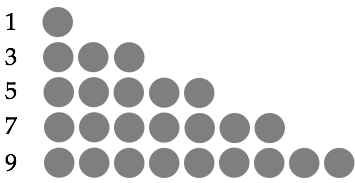
\includegraphics[scale=0.4]{FiguresMaths/SumOddsBasis}
\caption{Representing the first $n$ odd integers using tokens.  In this illustration, $n=5$.}
       \label{fig:sumOdds1}
\end{center}
\end{figure}

Starting with this picture, we take each row of $2i-1$ tokens and ``fold" it at its midpoint so that it becomes a reversed letter ``$L$''.  The row of $2i-1$ tokens becomes an ``$L$'' whose horizontal portion (at the bottom of the reversed ``$L$'') is a row of $i$ tokens and whose vertical portion (at the right of the reversed ``$L$'') is a column of $i$ tokens (the ``hinge" token resides in both portions).
\begin{figure}[ht]
\begin{center}
       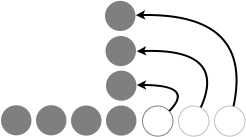
\includegraphics[scale=0.4]{FiguresMaths/SumOddsIntermediate}
              \caption{Folding a single row into a reversed letter ``$L$''.}
       \label{fig:sumOdds2}
\end{center}
\end{figure}

Once we have folded every row of tokens into a reversed ``$L$'', we nest the different-size occurrences of ``$L$'' into one another, in the manner depicted in Fig~\ref{fig:sumOdds3}.
\begin{figure}[ht]
\begin{center}
       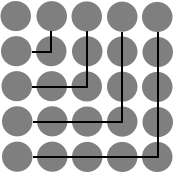
\includegraphics[scale=0.4]{FiguresMaths/SumOddsFinal}
\caption{The final picture organized as an $n \times n$ square array of tokens.}
       \label{fig:sumOdds3}
\end{center}
\end{figure}
Clearly, this nesting produces an $n \times n$ square array of (perforce, $n^2$) tokens.
\end{proof}

\medskip

\index{$n^2$ as sum of first $n$ odd integers!another proof ``by pictures''}
\begin{proof}
{\bf Another ``pictorial" proof.}
The reader who enjoyed the preceding ```pictorial' proof'' may be amused by the challenge of completing the kindred slightly more complex proof illustrated by Fig.~\ref{fig:anotherSumOdds}.
\begin{figure}[htb]
\begin{center}
       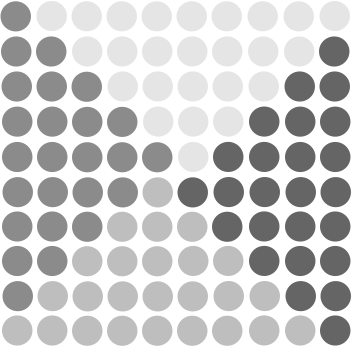
\includegraphics[scale=0.35]{FiguresMaths/Deltaodd}
\caption{Four copies of $S(n)$ represented as a triangle of tokens.  The triangles are arranged to yield a $2n \times 2n$ square of tokens.}
       \label{fig:anotherSumOdds}
\end{center}
\end{figure}
In the figure we have illustrate four copies of the triangle of tokens which depicts summation $S(n)$ (which sums the first $n$ odd numbers).  We have arranged the triangles in a way that produces a $2n \times 2n$ square of tokens.  In the arrangement, each side of the square is a line of $1+2n-1 \ = \ 2n$ tokens.  This construction illustrates that $4 S(n) \ = \ (2n)^2  \ = \ 4n^2$.
\end{proof}

\medskip

\noindent \fbox{
\begin{minipage}{0.96\textwidth}
{\bf Explanatory note}.

\textit{Full disclosure}: Fig.~\ref{fig:anotherSumOdds} provides the basis for a proof of 
Proposition~\ref{thm:squares-odd-integers-Gauss}, but it does not provide the complete proof: We must somehow verify that the construction in the figure is completely general, i.e., that the depicted emergence of the $2n \times 2n$ square of tokens from four copies of the $\Delta_n$-triangle is not an artifact of the depicted case $n =5$.  This verification is not difficult.

\medskip

What is notable about Fig.~\ref{fig:anotherSumOdds}, even with this caveat, is how it truly facilitates the {\em discovery} of the Proposition.

\medskip

Of course, it should not be surprising that pictorial reasoning is useful in highlighting the kinds of patterns that lead to discoveries as  we {\em do} mathematics.  It should also come as no surprise that nothing comes for free.  As this example indicates: Even when pictorial reasoning leads us to intriguing discoveries, it does not obviate the invocation of additional modalities of reasoning for rigorously verifying the facts that the patterns reveal.
\end{minipage}
}

\medskip

\ignore{********
{\Denis I added the following construction in the 2 figures, please, select the one you prefer.
If you think this result is too marginal here, we can put it as an exercice...}
This result can be obtained similarly by a slightly different arrangement by counting the tokens
of $4$ triangles representing the sum of the first $n$ integers $S(n)$ as shown in Fig~\ref{fig:alternateSumOdds}.
The side of the square is equal to $1+2n-1=2n$, thus $4 \cdot S(n)=(2n)^2= 4n^2$.

%\begin{figure}[ht]
%\begin{center}
%       
\includegraphics[scale=0.4]{FiguresMaths/DeltaoddSynthetic}
%\caption{Schematic view of how to obtain the $2n \times 2n$ square.}
%       \label{fig:alternateSumOdds2}
%\end{center}
%\end{figure}
***************}

\ignore{\Arny More calculation!  BOO!  Please complete this.  I seem to be off by 1}
%We give another proof that tells us something more on numbers of their interactions.
%We consider numbers instead of tokens, and we use a similar principle as Fubini, that is to determine a
%suitable organization of the numbers and count them in a simple way.
%For the concern of computing the sum of the first odd numbers, we organize them as shown in Table~\ref{tab:SumOddsTriangle}.
%One number in the first row, two in the second, $k$ on the $k$th row.
%There are $\Delta_p$ (complete) rows. 
%The result is obtained by summing up the elements of each row.
%The sum in a row is equal to the perfect cube of this row.
%This result can be easily proven. 
%{\Denis Should I develop here? or we can let it as an exercice?}
%

\bigskip

\noindent {\em A preview of coming attractions}.
In Section~\ref{sec:sum-of-i2c>0}, we develop the underpinnings of
techniques that incrementally compute:
\begin{itemize}
\item
the sums of the first $n$ consecutive integers (the summations $S_1(n)$), 
\item
the sums of the first $n$ squares of the integers (the summations $S_2(n)$), 
\item
the sums of the first $n$ cubes of the integers (the summations $S_3(n)$),
\end{itemize}
and so on.  We have, thus begun to establish a base for a summation technique that is {\em inductive}, i.e., that computes each summation $S_c(n)$ from the lower-index summations: $S_1(n)$, $S_2(n)$, \ldots, $S_{c-1}(n)$.  Our inductive technique awaits a bit more background.

%%%%%%%%%%%%%%%%%%%%%%%%%%%%%%%%%%%%%%%%%%%%%%%%%%%%

\subsection{Geometric Sums and Series}
\label{sec:general-geometric-series}
\label{sec:geometric-sums}
\label{sec:general-geometric-sums}

\subsubsection{Overview and main results}

We define geometric sequences and series and learn how to calculate their sums via the following generic examples.
\index{geometric sequence}
\index{geometric summations}
\index{geometric series}

\medskip

An $n$-term geometric sequence:
\begin{equation}
\label{eq:genl-geom-seq}
a, \ ab, \ ab^2, \ \ldots, ab^{n-1}
\end{equation}

The corresponding geometric summation:
\begin{eqnarray}
\label{eq:genl-geom-summation}
S_{a,b}(n)
 \ \eqdef \  \sum_{i=0}^{n-1} a b^i 
 & = &  a + ab + ab^2 + \cdots + ab^{n-1} \\
\nonumber
 & = & 
 a \cdot (1+ b + b^2 + \cdots + b^{n-1})
\end{eqnarray}

The associated geometric {\em (infinite) series} (used only when $b < 1$):
\begin{equation}
\label{eq:genl-geom-series}
S_{a,b}^{(\infty)} \ \ \eqdef \ \  \sum_{i=0}^\infty a b^i
 \ \  = \ \   a + ab + ab^2 + \cdots 
\end{equation}

\medskip

\noindent
Two related facts are clear from these definitions:

\noindent
We can evaluate the summation (\ref{eq:genl-geom-summation}) by evaluating just the sub-summation
\begin{equation}
\label{eq:geom-summation}
S_{b}(n) \ \eqdef \ \sum_{i=0}^{n-1} b^i \ = \ 1+ b + b^2 + \cdots + b^{n-1}
\end{equation}
We can evaluate the series (\ref{eq:genl-geom-series}) by evaluating just the sub-series
\begin{equation}
\label{eq:geom-series}
S_{b}^{(\infty)} \ \ \eqdef \ \ \sum_{i=0}^\infty b_i \ \ = \ \ 1+ b + b^2 + \cdots 
\end{equation}

\bigskip

\index{evaluating geometric sums and series}
This section's major results are embodied in the following proposition.

\begin{prop}
\label{thm:sum-finite-geometric-series}
Let $S_{b}(n)$ be a geometric summation, as defined in
(\ref{eq:geom-summation}).

\smallskip

\noindent {\bf (a)}
When $b > 1$, $S_{b}(n)$ evaluates to the following sum.
\begin{equation}
\label{eq:geom-sum:b>1}
S^{(b>1)}_{b}(n) \ = \ \frac{b^{n}- 1}{b - 1}
\end{equation}

\smallskip

\noindent {\bf (b)}
When $b < 1$, $S_{b}(n)$ evaluates to the following sum.
\begin{equation}
\label{eq:geom-sum:b<1}
S^{(b<1)}_{b}(n) \ = \ \frac{1 - b^n}{1-b}
\end{equation}

\smallskip

\noindent {\bf (c)}
In the uninteresting, {\em degenerate}, case $b=1$
\[ S^{(b=1)}_{b}(n) \ = \ 1 + 1 + \cdots + 1 \ \ \mbox{($n$ times)} \ \ = \ n \]
\end{prop}

\medskip

\index{degenerate cases in mathematics}

\noindent \fbox{
\begin{minipage}{0.96\textwidth}
{\bf Explanatory note \#1}.

Of course, the expressions (\ref{eq:geom-sum:b>1}) for $S^{(b>1)}_{b}(n)$ and (\ref{eq:geom-sum:b<1}) for $S^{(b<1)}_{b}(n)$ are algebraically equivalent as functions of $b$ and $n$.  But they will be read differently:
\[ \Big[ S^{(2)}_{2}(n) \ = \ 2^n -1 \Big] \ \ \ \
\mbox{ while } \ \ \ \
\left[ S^{(1/2)}_{2}(n) \ = \ \frac{ 1 - \left({1 \over 2} \right)^n}{ 1 - \left({1 \over 2} \right)} \ = \
2 - \left({1 \over 2} \right)^{n-1} \right] \]
\end{minipage} }

\index{degenerate cases in mathematics}
\bigskip

\index{degenerate cases in mathematics}

\noindent \fbox{
\begin{minipage}{0.96\textwidth}
{\bf Explanatory note \#2}.

The {\it New Oxford Dictionary} defines the word ``degenerate" as follows:

\smallskip

{\small
lacking some property, order, or distinctness of structure previously or usually present.

\smallskip

{\em Mathematics} relating to or denoting an example of a particular type of equation, curve, or other entity that is equivalent to a simpler type, often occurring when a variable or parameter is set to zero.
}

\medskip

In our case, the structures of the terms in summations (\ref{eq:geom-sum:b>1}) and (\ref{eq:geom-sum:b<1}) play a critical role in determining the sums of the summations.  In the case $b=1$, all terms lack structure: they ``degenerate" to value $1$.
\end{minipage}
}

\bigskip

The infinite case (\ref{eq:geom-series}) can be dealt with as a corollary of Proposition~\ref{thm:sum-finite-geometric-series}(b), by letting $n$ grow without bound and observing that the resulting sequence of values converges.

\begin{prop}
\label{thm:sum-infinite-geometric-series}
When $b < 1$,  the {\em infinite} series $S^{(\infty)}_{b}$ {\em
  converges} to the following sum.
\[ S^{(\infty)}_{b} \ \ = \ \
\sum_{i=0}^\infty \ b^i \ \ = \ \ 1 + b + b^2 + \cdots
 \ \ = \ \ \frac{1}{1-b}
\]
\end{prop}

\subsubsection{Techniques for summing geometric series}
\label{sec:summing-geometric-series:techniques}

We turn now to a sequence of proofs of Propositions~\ref{thm:sum-finite-geometric-series} and~\ref{thm:sum-infinite-geometric-series}.

\medskip

\index{evaluating geometric sums and series!by textual replication}
\begin{proof}
{\bf A proof via textual replication.}
Toward the end of developing our first method for summing $S_{b}(n)$, we note that we can rewrite the sum in two ways that are {\em (textually) recurrent}.

\bigskip

\noindent
This phenomenon of {\em finding recurrent subexpressions} is a ``pattern'' of the form described in Chapter~\ref{ch:doingmath}.  We now describe how this pattern can be exploited to find explicit sums for geometric summations and series.

\bigskip

\noindent
Both of the recurrent expressions for $S_{b}(n)$ have the form
\begin{equation}
\label{eq:geom-series-recurrent}
S_b(n) \ = \ \alpha \cdot S_b(n) \ + \ \beta(n)
\end{equation}
where $\alpha$ is a constant and $\beta(n)$ is a function of $n$; both $\alpha$ and $\beta(n)$ may depend on the parameter $b$.  We provide two recurrent expressions for $S_b(n)$, one of which is more interesting when $b>1$, the other when $b<1$.
\begin{eqnarray}
\label{eq:geom-series-replicate}
\nonumber
S_{b}(n) 
  & \eqdef &
1+ b + b^2 + \cdots + b^{n-1}  \\
\nonumber
  &   &  \\
\label{eq:geom-series-replicate-1}
   & = & b \cdot S_{b}(n) \ + \ (1 - b^n) \\
\nonumber
   &  & \\
\label{eq:geom-series-replicate-2}
  & = &
\frac{1}{b} \cdot S_{b}(n) \ + \ \frac{b^n -1}{b} 
\end{eqnarray}
The significance of a recurrent expression of the type (\ref{eq:geom-series-recurrent}) is that it exposes an explicit value for $S_b(n)$:
\begin{equation}
\label{eq:geom-series-generic}
S_b(n) \ = \ \frac{\beta(n)}{1 - \alpha}
\end{equation}

\medskip

We now combine the generic value (\ref{eq:geom-series-generic}) of $S_b(n)$ with the specialized recurrent expressions in (\ref{eq:geom-series-replicate-1}) and (\ref{eq:geom-series-replicate-2}) to derive two explicit solutions for $S_b(n)$.
\begin{enumerate}
\item
The first solution is most useful and perspicuous when $b>1$.  In this case:
\[ \left( 1 - \frac{1}{b} \right)  S^{(b>1)}_{b}(n) \ = \ b^{n-1} - \frac{1}{b} \]
which is easily rearranged to the equivalent and more perspicuous form (\ref{eq:geom-sum:b>1}).

\item
The second solution is most useful and perspicuous when $b < 1$.  In this case:
\[ (1-b) S^{(b<1)}_{b}(n) \ = \ 1 \ - \ b^n \]
which is easily rearranged to the equivalent and more perspicuous form (\ref{eq:geom-sum:b<1}).
\end{enumerate}
\end{proof}

\medskip

Note that both $S^{(b>1)}_{b}(n)$ and $S^{(b<1)}_{b}(n)$ have simple {\em approximate} values which are useful in ``back-of-the-envelope'' calculations: For very large values of $n$, we have
\begin{equation}
\label{eq:geom-sum:approx}
S^{(b>1)}_{b}(n) \ \approx \ \frac{b^n}{b-1} \ \ \ \
\mbox{and} \ \ \ \
S^{(b<1)}_{b}(n) \ \approx \ \frac{1}{1-b} 
\end{equation}
The expression for $S^{(b<1)}_{b}(n)$ in (\ref{eq:geom-sum:approx}) is actually a rewording of
Proposition~\ref{thm:sum-infinite-geometric-series}.

\medskip

\index{evaluating geometric sums and series!a pictorial way to sum $S^{(\infty)}_{1/2}$ using cascading shrinking squares}
\begin{proof}
{\bf A ``pictorial" summation of $S^{(\infty)}_{1/2}$.}
Fig.~\ref{fig:sumGeoBasis} pictorially depicts a process whose analysis provides a rigorous proof of Proposition~\ref{thm:sum-infinite-geometric-series} for the case $b = 1/2$, \textit{i.e.}, a rigorous argument that the series $S^{(\infty)}_{1/2} = \sum_{i=0}^\infty \ 2^{-i}$ sums to $2$.
\begin{figure}[htb]
\begin{center}
       \includegraphics[scale=0.35]{FiguresMaths/SumGeometric1sur2Bis}
 \caption{Arranging successive rectangles to evaluate $S^{(\infty)}_{1/2}$.}
       \label{fig:sumGeoBasis}
\end{center}
\end{figure}
In this evaluation of $S^{(\infty)}_{1/2}$, we measure fractional quantities by the portion of a unit-side rectangle that they fill.  Thus (follow in the figure): the initial term of $S^{(\infty)}_{1/2}$, namely, $1$, is represented by the unit square that is labeled ``$1$'' in the figure.  The next term of the series, namely, $1/2$, is represented by the rectangle labeled ``$1/2$'' in the figure.  And so on, with successively smaller rectangles.  Because we design each rectangle to have half the area of its predecessor, the sequence of rectangles represents successively smaller inverse powers of $2$.  As the process proceeds, we observe increasingly more of the righthand unit-side square being filled.  In fact, one can verify, via an elementary induction, that {\em every} point in the righthand unit-side square eventually gets covered by some small rectangle (as $n$ tends to $\infty$), thereby establishing that the infinite series $S^{(\infty)}_{1/2}$ does, indeed, sum to $2$.

\bigskip

The preceding procedure is difficult, but not impossible, to adapt to values of $b <1$ other than $1/2$.  The sequence Fig.~\ref{fig:sumGeoGeneral1}--Fig.~\ref{fig:sumGeoGeneral3}
\begin{figure}[htb]
\begin{center}
       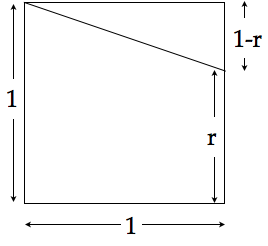
\includegraphics[scale=0.35]{FiguresMaths/SumGeometricGeneral1}
\caption{Initial state: the unit square and the base $b$.}
       \label{fig:sumGeoGeneral1}
\end{center}
\end{figure}
\begin{figure}[htb]
\begin{center}
       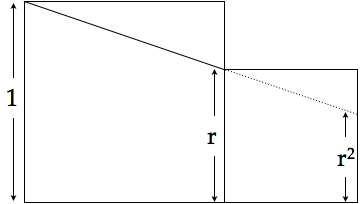
\includegraphics[scale=0.35]{FiguresMaths/SumGeometricGeneral2}
\caption{Beginning to develop the geometric series via cascading shrinking squares.}
       \label{fig:sumGeoGeneral2}
\end{center}
\end{figure}
suggests how to achieve such an adaptation for any value of $b$ with $0 \leq b <1$, via an appropriate cascade of shrinking squares.
\begin{figure}[ht]
\begin{center}
       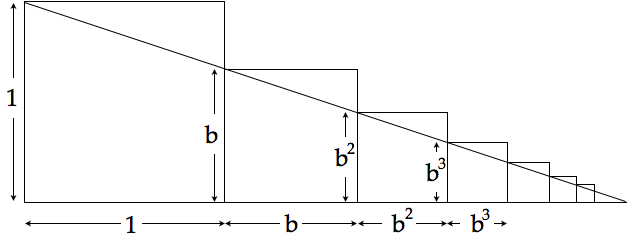
\includegraphics[scale=0.35]{FiguresMaths/SumGeometricGeneral3}
\caption{The complete process for computing a geometric series by using a cascade of shrinking squares.}
       \label{fig:sumGeoGeneral3}
\end{center}
\end{figure}
The unit-side square in Fig.~\ref{fig:sumGeoGeneral1} begins the construction of the cascade.  The two squares in Fig.~\ref{fig:sumGeoGeneral2} illustrate the second step in constructing the cascade; the suggestive cascade depicted in Fig.~\ref{fig:sumGeoGeneral3} illustrates what the final cascade looks like: The cumulative length of the bases of its abutting rectangles is the value of the infinite series $S_b^{(\infty)}$; cf.~(\ref{eq:genl-geom-series}).  The proof that the base of the cascade in the figure yields the desired sum is completed by a version of the theorem about similar triangles which is associated with Thales of Miletus and mentioned in Euclid's {\it Elements}. \qed
\end{proof}
\index{Thales of Miletus} \index{Euclid}

\medskip

\noindent \fbox{
\begin{minipage}{0.96\textwidth}
{\bf Explanatory/historical note.}

Thales of Miletus is credited with a classical theorem about similar right triangles.  The following figure depicts right triangle $T$ and its (shaded) sub-triangle $T'$ whose right angle is distance $1$ from $T$'s.

\begin{center}
       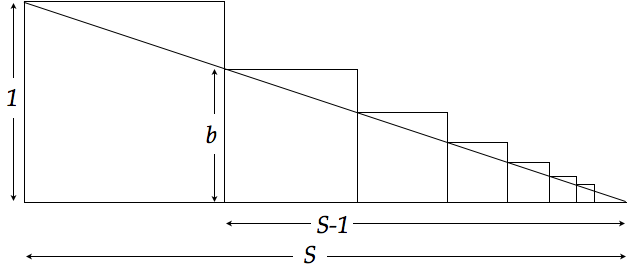
\includegraphics[scale=0.3]{FiguresArithmetic/ThalesGeometricSum}
\end{center}

\begin{prop}[The Theorem of Thales]
\label{thm:Thm-of-Thales-similarity}
Let us be given a unit-height right triangle $T$ whose base has length $S$.  The ratio $(S-1)/S$  equals the height $b$ of the sub-triangle $T'$ whose right angle is at distance $1$ from $T$'s.
\end{prop}

We use this proportionality of the side-ratios of the big and small triangles to evaluate the summation $\sum_{i=0}^\infty \ b^{-i}$.
\end{minipage}
}

\ignore{***********
{\Denis We should add a final remark here}.
The final touch is that the infinite sum is given by the base of the big right rectangle.
It is similar ({\Denis we call this property semblable in french}) to the little right rectangle top left in the figure.
By Thales theorem in geometry, the ratio of the sides are proportional:
$\frac{S^{(\infty)}_{b} }{1} = \frac{1}{1-b}$. 
***********}

\medskip

%{\Denis We can add here two exercices.}
\ignore{************
{\Denis(1) I really like including the pie-cutting in the text,
  because it is another representation for exactly the same problem.
  Do you like this way of handling it?  
  YES
  (2) I am less enthusiastic
  about including the nexted triangles: it changes the problem (i.e.,
  the base b) as well as the representation.  
  OK, base b is somehow a generalization...
  I like it very much as
  an exercise ... but we have not yet tackled that issue.
  How the exercices will be included?}
**********}


\index{evaluating geometric sums and series!a pictorial way to sum $S^{(\infty)}_{1/2}$}
\begin{proof}
{\bf Another ``pictorial" summation of $S^{(\infty)}_{1/2}$.}
The pictorial derivation of the sum $S^{(\infty)}_{1/2}$ can be accomplished using geometric shapes other than squares.  We now present a natural derivation of the sum $S^{(\infty)}_{1/2}$ by vigorously slicing a pie.

The process of pie-slicing works most naturally with the modified series
\[ \overline{S}^{(\infty)}_{1/2} \ \ = \ \ \sum_{i=1}^\infty 2^{-i}
 \ \ = \ \ S^{(\infty)}_{1/2} \ - \ 1. \]
which omits the initial summand $1$ from $S^{(\infty)}_{1/2}$.  Of course, $\overline{S}^{(\infty)}_{1/2}$ sums to $1$, because $S^{(\infty)}_{1/2}$ sums to $2$.

\medskip

The pie-slicing evaluation of $\overline{S}^{(\infty)}_{1/2}$ is depicted in Fig~\ref{fig:sumGeo1sur2circle}.  In the figure, the inverse powers of $2$ are represented by appropriate fractions of a unit-diameter disk (the pie).  The evaluation begins with this disk before it is sliced: this represents the number $1$, which we eventually show to be the sum
$\overline{S}^{(\infty)}_{1/2}$.
\begin{figure}[htb]
\begin{center}
       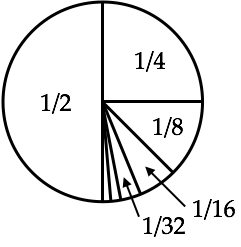
\includegraphics[scale=0.35]{FiguresMaths/SumGeometric1sur2circle}
\caption{Computing the sum of $1/2^i$ by slicing a unit disk.}
       \label{fig:sumGeo1sur2circle}
\end{center}
\end{figure}
We slice the disk in half using the depicted diameter and label one of the resulting half-disks ``$1/2$''.  Next, we slice one of the half-disks in half using a radius of the unit disk and label one of the quarter-disks ``$1/4$''.  We continue in this manner {\em ad infinitum}.  The analysis that yields the sum $\overline{S}^{(\infty)}_{1/2}$ amounts to a proof that every point in the unit-diameter disk eventually resides in a slice that is not further sliced.  Details are left to the reader.  \qed
\end{proof}


\subsubsection{Extended geometric series and their sums}
\label{sec:extended-geom-series}
\index{extended geometric sums: $\sum_{i=1}^n \ i^c b^i$}

We now build on our ability to evaluate geometric summations of the forms (\ref{eq:geom-sum:b>1}) and (\ref{eq:geom-sum:b<1}) to evaluate summations that we term {\em extended} geometric summations (not a standard term), i.e., summations of the form
\[ S_b^{(c)}(n) \ \eqdef \ \sum_{i=1}^n \ i^c b^i, \]
where $c$ is an arbitrary fixed positive integer, and $b$ is an arbitrary fixed real number.

\smallskip

We restrict attention in this section to summations $S_b^{(c)}(n)$ that satisfy the joint inequalities $c \neq 0$ and $b \neq 1$.

\medskip

\begin{itemize}
\item
We have already adequately studied the case $c=0$, which characterizes ``ordinary'' geometric summations.
\item
The degenerate case $b = 1$ removes the ``geometric growth'' of the sequence underlying the summation.  We study various aspects of this {\it summation-of-fixed-powers} case in Section~\ref{sec:smooth-series}, with special treatment of summations of fixed powers of consecutive integers in Section~\ref{sec:sum-of-i2c}.
\end{itemize}

\medskip

The summation method that we now develop for evaluating all other summations $S_b^{(c)}(n)$---i.e., those with $b \neq 1$ and $c \neq 0$---has the following notable properties.
\begin{itemize}
\item
The method is {\em inductive in parameter} $c$.

\smallskip

Specifically, we will express our sum for $S_b^{(c)}(n)$ in terms of sums for summations $S_b^{(c-1)}(n)$, $S_b^{(c-2)}(n)$, \ldots, $S_b^{(1)}(n)$, and $S_b^{(0)}(n) = S_b(n)$.

\item
For each fixed value of $c$, the method is {\em inductive in the argument} $n$.

\item
The method relies on the recurrent-subexpression strategy which we used effectively in Section~\ref{sec:general-geometric-sums}.
\end{itemize}

\medskip

\index{extended geometric sums: $\sum_{i=1}^n \ i^c b^i$!the case $c=1$}
\paragraph{A. The summation $S^{(1)}_b(n) = \sum_{i=1}^n i b^i$}

We illustrate our strategy in detail for the case $c=1$ and sketch only briefly how it deals with larger values of $c$.  Elementary algebraic manipulations which are suggested by the analysis of the case $c=1$ should thereby allow the reader to deal with any value $c > 1$.

\begin{prop}
\label{thm:sum-i2i}
For all bases $b > 1$,
\begin{equation}
\label{eq:sum-i2i}
S_b^{(1)}(n) \ \ = \ \
\sum_{i=1}^n \ i b^i
\ \ = \ \ 
\frac{(b-1)n -1}{(b-1)^2} \cdot  b^{n+1} \ + \ \frac{b}{(b-1)^2}
\end{equation}
\end{prop}

\index{extended geometric sums: $\sum_{i=1}^n \ i^c b^i$!the case $c=1$!summing via algebraic manipulation}
\begin{proof}
{\bf Deriving a sum via algebraic manipulation.}
We begin to develop our strategy by writing the natural expression for
\[ S_b^{(1)}(n) \ \ = \ \ b \ + \ 2b^2 \ + \ 3 b^3 \ + \cdots + \ n b^n  \]
in two different ways.  First, we isolate the summation's last term:
\begin{equation}
\label{eq:ext-geom-c=1.1}
S_b^{(1)}(n+1) \ = \ S_b^{(1)}(n) \ + \ (n+1) b^{n+1}
\end{equation}
Then we isolate the lefthand side of (\ref{eq:ext-geom-c=1.1}):
\begin{eqnarray}
\nonumber
S_b^{(1)}(n+1)
     & = &
b + \sum_{i=2}^{n+1} \ i b^{i}  \\
\nonumber
& = &
b + \sum_{i=1}^n \ (i+1) b^{i+1}  \\
\nonumber
     & = &
b +  b \cdot \sum_{i=1}^n \ (i+1) b^i \\
\nonumber
     & = &
b + 
b \cdot \left(
\sum_{i=1}^n \ i b^i 
 \ + \
\sum_{i=1}^n \  b^i 
\right) \\
\nonumber
     & = &
b \cdot \left( S_b^{(1)}(n) \ + \ S_b^{(0)}(n) \right) \ + \ b \\
\nonumber
& = &
b \cdot \left( S_b^{(1)}(n) \ +  \frac{b^{n+1} -1}{b-1} -1 \right) \ + \ b \\
\label{eq:ext-geom-c=1.2}
    & = &
b \cdot S_b^{(1)}(n) \ + \ b \cdot \frac{b^{n+1} - 1}{b-1}
\end{eqnarray}
Combining expressions (\ref{eq:ext-geom-c=1.1}) and (\ref{eq:ext-geom-c=1.2}) for $S_b^{(1)}(n+1)$, we finally find that
\begin{eqnarray}
\nonumber
(b-1) \cdot S_b^{(1)}(n) & = &
(n+1) \cdot b^{n+1} \ - \ b \cdot \frac{b^{n+1} -1}{b-1} \\
\label{eq:sum-i2i-source}
 & = &
\left( n - \frac{1}{b-1} \right) \cdot b^{n+1} \ + \ \frac{b}{b-1}
\end{eqnarray}
We now use standard algebraic manipulations to derive expression (\ref{eq:sum-i2i}) from equation (\ref{eq:sum-i2i-source}).  \qed
\end{proof}

\index{extended geometric sums: $\sum_{i=1}^n \ i^c b^i$!the case $c=1$!solving the case $b=2$ using subsum rearrangement}
\begin{proof}
{\bf Solving the case $b=2$ using subsum rearrangement.}
We evaluate the sum
\[
S_2^{(1)}(n) \ = \ \sum_{i=1}^n \ i 2^i
\]
in an especially interesting way, by rearranging the sub-summations of the target summation.

\bigskip

\noindent \fbox{
\begin{minipage}{0.96\textwidth}
{\bf Explanatory note}.

The reader should pay careful attention to this technique.  It shows that one can sometimes decompose a cumbersome expression for a summation into a readily manipulated one.
\end{minipage}
}

\bigskip

Underlying our evaluation of $S_2^{(1)}(n)$ is the fact that we can rewrite the summation as a {\em double} summation:
\begin{equation}
\label{eq:geom-double-sum}
S_2^{(1)}(n) \ = \ \sum_{i=1}^n \ \sum_{k=1}^{i} 2^i
\end{equation}

By suitably applying the laws of arithmetic that appear in Section~\ref{sec:Arithmetic-Laws}---specifically, the distributive, associative, and commutative laws---we can perform the required double summation in a different order than that specified in (\ref{eq:geom-double-sum}).  In fact, we can exchange the indices of summation in a manner that enables us to compute $S_2^{(1)}(n)$ in the order implied by the following expression:
\[
S_2^{(1)}(n) \ = \ \sum_{k=1}^{n} \ \sum_{i=k}^{n} 2^i
\]
This process is depicted in Fig.~\ref{fig:Sumi2i}.
\begin{figure}[htb]
\centerline{
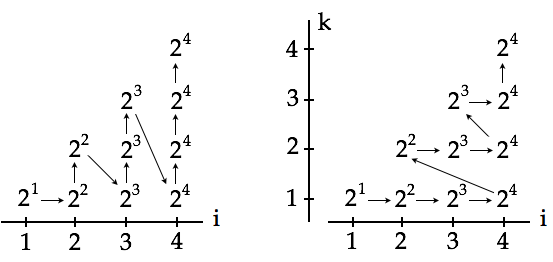
\includegraphics[scale=0.35]{FiguresMaths/Sumi2i}
}
\caption{Illustrating the case $n=4$ of the exchange of indices in the summation.  The original summation is drawn on the left.  In the righthand drawing, we reproduce each term $i \cdot 2^i$ $i$ times within column $i$.  We then express the summation on the right by introducing a new index $k$ and scanning the terms of the summation row by row (on the right).  The arrows represent the flow of the scan.}
\label{fig:Sumi2i}
\end{figure}
The indicated summation is much easier to perform in this order,
because its core consists of instances of the ``ordinary'' geometric
summation $\sum_{i=k}^{n} 2^i$ (Proposition~\ref{thm:sum-finite-geometric-series}).  Expanding these instances, we find finally that
\begin{eqnarray*}
S_2^{(1)}(n)
  & = &
\sum_{k=1}^{n} \ \big( 2^{n+1} -1 - \sum_{i=0}^{k-1} \ 2^i \big) \\
  & = &
\sum_{k=1}^{n} \ \big( 2^{n+1} - 2^k \big) \\
  & = &
n \cdot 2^{n+1}\ - ( 2^{n+1} -1) +1 \\
  & = &
(n-1) \cdot 2^{n+1} +2
\end{eqnarray*}
This completes the proof.  \qed
\end{proof}

We remark that the process of obtaining the original summation can also be seen in the figure, by scanning the elements of the summation along diagonals, as depicted in Fig.~\ref{fig:Sumi2iDiag}.  Each of the $n$ diagonals contains exactly the difference between the
complete geometric summation and the partial summation that is truncated at the $k$th term.
\begin{figure}[htb]
\centerline{
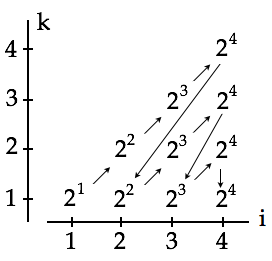
\includegraphics[scale=0.35]{FiguresMaths/Sumi2iDiag}
}
\caption{The successive diagonal patterns correspond to the single summation obtained after exchanging the two initial sums.}
\label{fig:Sumi2iDiag}
\end{figure}


\paragraph{B. The summations $S^{(c)}_b(n) =  \sum_{i=1}^n i^c b^i$}

We now develop a strategy which adapts the evaluation of summation $S_b^{(1)}(n)$ in the proof of Proposition~\ref{thm:sum-i2i} to an evaluation of the general extended geometric summation
\[
S_b^{(c)}(n) \ \ = \ \ \sum_{i=1}^n \ i^c b^i
 \ \ = \ \
b \ + \ 2^{c} b^2\ + \ 3^{c} b^3 \ + \ \cdots \ + \ n^{c} b^{n}
\]
The strategy is {\em recursive}, in that it computes a value for $S^{(c)}_b(n)$ from values for $S^{(c-1)}_b(n)$, $S^{(c-2)}_b(n)$, \ldots, $S^{(0)}_b(n)$.  It proceeds in three steps.

\smallskip

\noindent {\bf Step 1.}
As in the case $c=1$, we write summation $S_b^{(c)}(n)$ in two ways.  The expression that embodies the first way isolates the summation's first term:
\[ S_b^{(c)}(n+1) \ = \ b + \sum_{i=1}^n \ (i+1)^c b^{i+1} \]
The expression that embodies the second way isolates the summation's last term:
\[ S_b^{(c)}(n+1) \ = \ S_b^{(c)}(n) \ + \ (n+1)^{c} b^{n+1} \]
By combining these expressions, we find that
\begin{equation}
\label{eq:Sbcn-1}
S_b^{(c)}(n) 
 \ = \
b \cdot \left(
1 \ - \
(n+1)^{c} b^{n} \ + \
 \sum_{i=1}^n \ (i+1)^c b^{i} 
\right)
\end{equation}

\smallskip

\noindent {\bf Step 2.}
We next invoke the Restricted Binomial Theorem (Theorem~\ref{thm:restricted-binomial-thm}) to see that
\[ (i+1)^c \ = \ i^c \ + \ c \cdot i^{c-1} \ + \ {c \choose 2} \cdot
i^{c-2} \ + \cdots + \ {c \choose k} \cdot i^{c-k}  \ + \cdots + \ 1
\]

We use this expansion of $(i+1)^c$, together with multiple applications of the laws of arithmetic from Section~\ref{sec:Arithmetic-Laws} to verify that
\begin{eqnarray}
\nonumber
\sum_{i=1}^n \ (i+1)^c b^{i} & = &
S_b^{(c)}(n)
 \ + \ c \cdot S_b^{(c-1)}(n)
 \ + \ {c \choose 2} \cdot S_b^{(c-2)}(n)  \ + \cdots \\
\label{eq:Sbcn-2}
  &  & \cdots + \
{c \choose k} \cdot S_b^{(c-k)}(n)
 \ + \cdots + \
S_b^{(0)}(n)
\end{eqnarray}

\smallskip

\noindent {\bf Step 3.}
%
We finally combine equations (\ref{eq:Sbcn-1}) and (\ref{eq:Sbcn-2}) to discover that
\begin{eqnarray}
\nonumber
(b-1) \cdot S_b^{(c)}(n)
 & = &
(n+1)^{c} b^{n} \ - \
c \cdot S_b^{(c-1)}(n)
 \ - \ {c \choose 2} \cdot S_b^{(c-2)}(n)  \ - \cdots \\
\label{eq:Sbcn-3}
  &  & 
\cdots - \
{c \choose k} \cdot S_b^{(c-k)}(n)
 \ - \cdots - \
S_b^{(0)}(n)
\ - \ 1
\end{eqnarray}

We now have the promised method of evaluating the summation $S_b^{(c)}(n)$ associated with the fixed power $c$ in terms of the sums of kindred summations associated with smaller fixed powers.

\bigskip

Each incremental step in our summation technique is an elementary application of an idea that we have seen previously.  Careful pattern-matching---primarily always focusing on the ``top-level" of the target summation, i.e., on the largest current values of parameters $b$ and $c$---has enabled us to achieve a decidedly non-elementary goal via a sequence of elementary steps.

%%%%%%%%%%%%%%%%%%%%%%%%%%%%%%%%%%%%%%%%%

\section{On Summing ``Smooth'' Series}
\label{sec:smooth-series}

\subsection{Approximate Sums via Integration}
\label{sec:riemann-bounds}

This section develops and illustrates a powerful strategy for obtaining nontrivial upper and lower bounds on the sums of summations and series, by finding continuous {\em envelopes} that bound the summations both above and below.  The areas under the enveloping continuous functions---which we can calculate via integration---provide the desired bounds on the summations.

\medskip

The stratagem follows a three-step procedure.  Focus on a summation
\[ S \ = \ a_1 \ + \ a_2 \ + \ \cdots \ + \ a_n \]
whose sum we want to determine.  We have specified $S$ as a {\em finite} summation to simplify exposition; our stratagem often works with infinite summations also, as we shall see via specific examples.

\medskip

\noindent {\bf Step 1.}
Represent the summands of $S$ seriatim as $n$ abutting unit-width rectangles of respective heights $a_1, \ a_2, \ldots, \ a_n$.  


\medskip

\noindent {\bf Step 2.}
Construct a continuous curve $\overline{C}(x)$ that passes through the corners of the unit-width rectangles specified by the summation, in such a way that the rectangles lie completely within the area under $\overline{C}(x)$.

\medskip

\noindent
Because the aggregate areas of the abutting rectangles lie completely under curve $\overline{C}(x)$, the area under the curve---obtained by integrating $\overline{C}(x)$ between appropriate limits---yields an {\em upper bound} on the value of the summation of interest.

\medskip

\noindent {\bf Step 3.}
Construct a continuous curve $\underline{C}(x)$ that passes through the corners of the unit-width rectangles specified by the summation, in such a way that the area under $\underline{C}(x)$ lies completely within the rectangles.

\medskip

\noindent
Because the area under the curve $\underline{C}(x)$ lies completely within the abutting rectangles, the area under the curve---obtained by integrating $\underline{C}(x)$ within appropriate limits---yields a {\em lower bound} on the summation of interest.

\bigskip

\noindent
We now describe two specific summations, to illustrate the stratagem in action.

\begin{enumerate}
\item
Fig.~\ref{fig:riemann-n2} illustrates our stratagem applied to the seven-term version of the summation $S_2(n) = \sum_{i=1}^n i^2$, namely,
\[ S_2(7) \ = \ 1 \ + \ 4 \ + \ 9 \ + \ 16 \ + \ 25 \ + \ 36 \ +  49 \]
The figure represents the terms of $S_2(7)$ by means of seven abutting unit-width rectangles whose respective heights are given by the terms.  The sum of $S_2(7)$ is, then, given by the aggregate area of the abutting rectangles.  If we were to extend the figure rightward---which increases $n$ and thereby extends the summation by encompassing more addends---then the next two rectangles would have respective heights $64$ and $81$.

\smallskip

Our stratagem mandates embellishing the rectangles in Fig.~\ref{fig:riemann-n2} by two continuous curves---labeled $\overline{C}$ and $\underline{C}$ in the figure---that connect the upper corners of the rectangles.
\begin{figure}[htb]
\centerline{
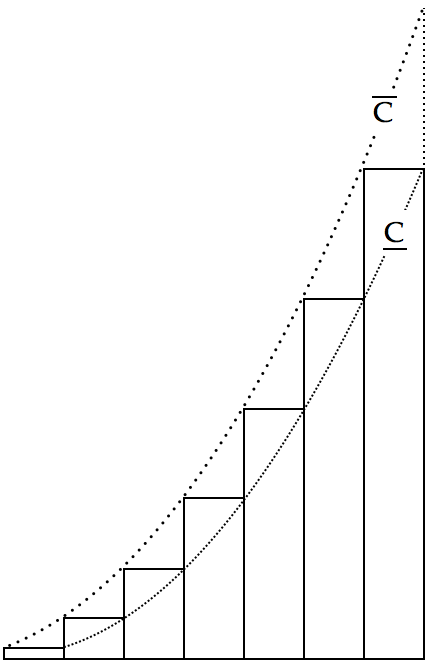
\includegraphics[scale=0.3]{FiguresMaths/SumSquaresContinuous}
}
\caption{The summation $S_2(n) = \sum_{i=1}^n i^2$ represented as the aggregate area of a sequence of unit-width shaded rectangles.  The summation is {\em bounded from above} by the area under the continuous curve $\overline{C}(x)$ that connects the upper lefthand corners of the rectangles; this curve is labeled $\overline{C}$ in the figure.  In detail, curve $\overline{C}$ begins at the upper lefthand corner of the leftmost rectangle; it continues to what would be the upper lefthand corner of the rightmost rectangle.  The area under curve $\overline{C}$ is $A(\overline{C}(x)) = \int_0^n \ (x+1)^2 dx$.  The summation is {\em bounded from below} by the area under the continuous curve $\underline{C}(x)$ that connects the upper righthand corners of the rectangles; this curve is labeled $\underline{C}$ in the figure.  In detail, curve $\underline{C}$ begins at the upper righthand corner of the leftmost rectangle; it continues to the upper righthand corner of the rightmost rectangle.  The area under curve $\underline{C}$ is $A(\underline{C}(x)) = \int_1^n \ x^2 dx$.}
\label{fig:riemann-n2}
\end{figure}
Curve $\overline{C}$ completely ``covers'' the rectangles; therefore, the area $A(\underline{C})$ under the curve is an {\em upper bound} on the aggregate area of the rectangles:
\[ A(\overline{C}(x)) \ = \ \int_1^n \ x^2 dx \]
Curve $\underline{C}$ lies completely within the rectangles; therefore, the area $A(\underline{C})$ under the curve is a {\em lower bound} on the aggregate area of the rectangles:
\[ A(\underline{C}(x)) \ = \  \int_0^{n-1}  \ x^2 dx \]

\item
Fig.~\ref{fig:riemann-harmonic} illustrates our stratagem as it applies to the ten-term version of the {\em harmonic} summation \index{harmonic sum}
\[ S^{(H)}(10) \ = \ \sum_{i=1}^{10} \ i^{-1} \ = \ \sum_{i=1}^{10} \ 1/i 
  \ = \
1 +  {1 \over 2} + {1 \over 3}  + {1 \over 4}  + {1 \over 5} + {1 \over 6} + {1 \over 7} + {1 \over 8}  + {1 \over 9}  + {1 \over 10} 
\]
The figure represents these terms via ten abutting unit-width rectangles whose respective heights are given by the terms.  The sum of $S^{(H)}(7)$ is, then, the aggregate area of the abutting rectangles.  If we were to extend the figure rightward (which increases $n$ and thereby extends the summation to encompass more addends), then the next two rectangles would have respective heights $1/11$ and $1/12$.

\smallskip

Our stratagem mandates embellishing the rectangles in Fig.~\ref{fig:riemann-harmonic} by two continuous curves---labeled $\overline{C}$ and $\underline{C}$ in the figure---that connect the rectangles' upper corners.
\begin{figure}[htb]
\centerline{
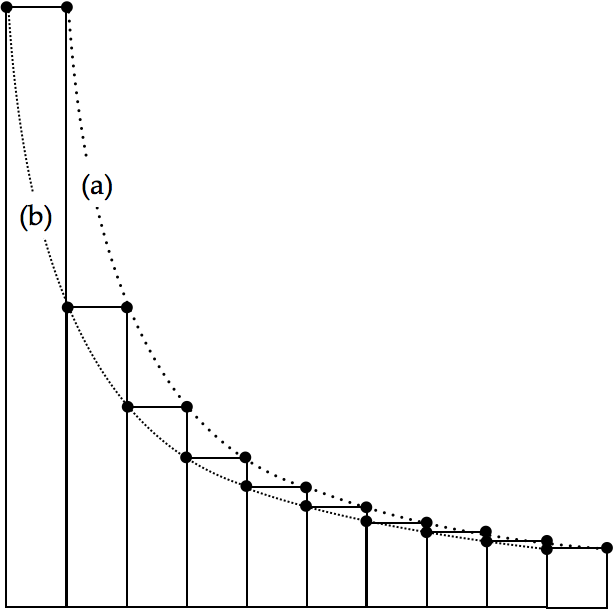
\includegraphics[scale=0.3]{FiguresMaths/RiemannSum}
}
\caption{The summation $S^{(H)}(n) \ = \ \sum_{i=1}^n \ 1/i$ represented as the aggregate area of a sequence of unit-width rectangles.  The summation is {\em bounded from above} by the area of the leftmost rectangle {\em plus} the area $A(\overline{C}(x))$ under the continuous curve $\overline{C}$ that connects the upper righthand corners of the rectangles.  In detail, this curve begins at the upper righthand corner of the leftmost rectangle; it continues to the upper righthand corner of the rightmost rectangle.  (The figure's resolution makes the righthand end of the curve invisible.)  The upper-bounding area is $A(\overline{C}(x)) = 1 \ + \ \int_1^n \ 1/x dx$.  The summation is {\em bounded from below} by the area $A(\underline{C}(x))$ under the continuous curve $\underline{C}$ that connects the upper lefthand corners of the rectangles.  In detail, curve $\underline{C}$ begins at the upper lefthand corner of the leftmost rectangle and continues to the upper lefthand corner of the rightmost rectangle.  The lower-bounding area is $A(\underline{C}(x)) =  \int_0^n \ 1/(x+1) dx$.}
\label{fig:riemann-harmonic}
\end{figure}
The lefthand rectangle {\em plus} curve $\overline{C}$ completely ``cover'' the rectangles; therefore, their combined areas provide an {\em upper bound} on the aggregate area of the rectangles.  Curve $\underline{C}$ lies completely within the rectangles; therefore, the area $A(\underline{C}(x))$ under the curve is a {\em lower bound} on the aggregate area of the rectangles.
\end{enumerate}

\bigskip

\noindent \fbox{
\begin{minipage}{0.96\textwidth}
{\bf Explanatory note}.

The curves labeled $\overline{C}$ in Figs.~\ref{fig:riemann-n2} and~\ref{fig:riemann-harmonic} are instances of the stratagem's mandated continuous curve $\overline{C}(x)$.  {\em Note that curve $\overline{C}$ in Fig.~\ref{fig:riemann-harmonic} must be considered to contain the top of the leftmost rectangle in the figure.}

\smallskip

The curves labeled $\underline{C}$ in Figs.~\ref{fig:riemann-n2} and~\ref{fig:riemann-harmonic} are instances of the stratagem's mandated continuous curve $\underline{C}(x)$. 
\end{minipage}
}

\bigskip

In the next subsection, we apply our stratagem to summations of fixed powers of successive integers, i.e., summations of the form
\[ S_c(n) \eqdef \sum_{i=1}^n i^c \]
for various (classes of) values of the fixed power $c$.


\subsection{Sums of Fixed Powers of Consecutive Integers: $\sum i^c$}
\label{sec:sum-of-i2c}

We derive bounds on the summations $S_c(n)$ which are rather good for large $n$.  In some cases, the bounds are very good, sometimes even exact for all $n$.

\subsubsection{$S_c(n)$ for general {\em nonnegative} real $c$th powers}
\label{sec:sum-of-i2c>0}

We begin to illustrate the technique of bounding summations via integrals by focusing on summations of the form
\[ S_c(n) \ \eqdef \ \sum_{i=1}^n \ i^c \]
for arbitrary positive numbers $c$.  The reader can garner intuition for the upcoming bounds from the general shapes of the continuous curves that rest upon the rectangles in Fig.~\ref{fig:riemann-n2}.  The bounds that we describe now can be specified more elegantly using the formalism which awaits us in Section~\ref{sec:asymptotics}.

\medskip

We obtain our bounds on each summation $S_c(n)$ by evaluating the integrals that yield the area $\overline{C}_c(n)$ under the continuous curve $\overline{C}$ in Fig.~\ref{fig:riemann-n2} and the area $\underline{C}_c(n)$ under the continuous curve $\underline{C}$ in the figure.  We thereby find that, for all sufficiently large $n$:
\begin{itemize}
\item
the former bound is given by
\begin{equation}
\label{eq:upper-integral-xc}
\overline{C}_c(n) \ = \
\int_0^n \ (x+1)^c dx \ = \
 \frac{1}{c+1} (n+1)^{c+1} \ + \ \overline{\kappa}
\end{equation}

\item
the latter bound is given by
\begin{equation}
\label{eq:lower-integral-xc}
\underline{C}_c(n) \ = \
\int_1^n \ x^c dx \ = \ \frac{1}{c+1} n^{c+1} \ + \ \underline{\kappa}
\end{equation}
\end{itemize}
The terms $\overline{\kappa}$ and $\underline{\kappa}$ are real constants which do not depend on $n$---although they could depend on $c$.

\smallskip

In order to combine the bounds (\ref{eq:upper-integral-xc}) and (\ref{eq:lower-integral-xc}) into a perspicuous two-sided bound for $S_c(n)$, we remark that there exists a constant $\kappa$ which does not depend on $n$---although it could depend on $c$---such that
\[ \frac{1}{c+1} n^{c+1} \ + \ \underline{\kappa} \ \leq \ \kappa n^c \]
{\em (We leave this verification to the reader.)}  With this final bound in hand, we finally have the sought two-sided bound on $S_c(n)$:

\begin{prop}
There exist constants $\overline{\kappa}$ and $\kappa$ which do not depend on $n$---although they could depend on $c$---such that, for all sufficiently large $n$:
\begin{equation}
\label{eq:bounds-sum-xc}
\frac{1}{c+1} n^{c+1} \ + \ \overline{\kappa}
  \ \ \leq \ \ S_c(n)
  \ \ \leq \ \ \frac{1}{c+1} n^{c+1} \ + \ \kappa n^c
\end{equation}
\end{prop}

\medskip

\noindent
The main message here is that when one views each $S_c(n)$ as a function of $n$:

\smallskip

\begin{center}
{\em The behavior of $S_c(n)$ is dominated by \ \
  $\displaystyle \frac{1}{c+1} n^{c+1}$ \ \ as $n$ grows without bound.  }
\end{center}

\subsubsection{Nonnegative integer $c$th powers}
\label{sec:positive-integer-power}

\paragraph{A. A better bound via the Binomial Theorem}

\index{The Binomial Theorem!restricted form}
When $c$ is a positive integer, the following special case of Newton's {\it Binomial Theorem}\footnote{The general form of the Binomial Theorem expands the polynomial $(x+y)^k$ rather than $(x+1)^k$; see Section~\ref{sec:Binomial-thm}.}~affords us a much more detailed upper bound on the sum of $S_c(n)$.

\begin{theorem}[The Restricted Binomial Theorem]
\label{thm:restricted-binomial-thm}
For all positive integers $k$,
\begin{equation}
\label{eq:restricted-binomial-thm}
(x+1)^k \ = \ \sum_{i=0}^k \ \ {k \choose i} x^{k-i}
\end{equation}
\end{theorem}

We improve our upper bound on $S_c(n)$ by paralleling the reasoning that led us to the relation (\ref{eq:upper-integral-xc}).  Our improved bound emerges also by evaluating the integral that
yields the area $\overline{C}_c(n)$ under the continuous curve that passes through the upper lefthand corners of the unit-width rectangles specified by summation $S_c(n)$.  For sufficiently large $n$:
\begin{eqnarray}
\label{eq:upper-integral-xk}
\overline{C}_c(n) \ = \
\int_0^n \ (x+1)^c dx & = &
\int_0^n \ \left(\sum_{i=0}^c \ \ {c \choose i} x^{c-i} \right) dx \\
\nonumber
& = &
\sum_{i=0}^c \left( \int_0^n \  {c \choose i} x^{c-i} \right) dx \\
\nonumber
  & = &
\sum_{i=0}^c \ \ \frac{1}{c-i+1} {c \choose i} n^{c-i+1} \ + \overline{\kappa}
\end{eqnarray}
where $\overline{\kappa}$ is our now-familiar unspecified fixed constant.  This is a proper upper bound because the region defined by this curve totally contains the region subtended by the rectangles.

\smallskip

Using this strategy, we find that for any positive integer $c$, summation $S_c(n)$ enjoys the following two-sided bound. For sufficiently large $n$:
\begin{equation}
\label{eq:bounds-sum-xk}
\frac{1}{c+1} n^{c+1} \ + \ \overline{\kappa}
  \ \ \leq \ \ \sum_{i=1}^n \ i^c
  \ \ \leq \ \ 
\sum_{i=0}^c \ \ \frac{1}{c-i+1} {c \choose i} n^{c-i+1} \ + \ \underline{\kappa}
\end{equation}
where $\overline{\kappa}$ and $\underline{\kappa}$ are fixed constants.

\smallskip

We have, of course, not changed the dominant behavior of $S_c(n)$ as $n$ grows without bound, but we have taken a significant step toward developing explicit expressions for the sums of the summations $S_c(n)$ when $c$ is a positive integer.

\paragraph{B. Using {\em undetermined coefficients} to refine sums}

\index{Method of Undetermined Coefficients}
We now introduce the {\em Method of Undetermined Coefficients} and illustrate its use in deriving explicit expressions for the sums $S_c(n)$ when $c$ is a positive integer.  Our development builds on the intuition (garnered from the bounds (\ref{eq:bounds-sum-xk})) that
\[ S_c(n) \ = \ \frac{1}{c+1} n^{c+1} \ + \ a^{(c)}_c n^c \ + \
a^{(c)}_{c-1} n^{c-1} \ + \ \cdots \ + \ a^{(c)}_2 n^2 \ + \ a^{(c)}_1 n
 + \ a^{(c)}_0
\]
for some nonnegative numbers $a^{(c)}_c$, \ldots, $a^{(c)}_0$.  To begin, we know that $a^{(c)}_0 = 0$, because $S_c(0) = 0$.

\bigskip

\noindent \fbox{
\begin{minipage}{0.96\textwidth}
{\bf Explanatory note}.

Because our starting point is a conjecture based only on intuition, we will have to verify the explicit expressions that we derive.  We do this after deriving the expressions.
\end{minipage}
}
\bigskip

The Method becomes computationally cumbersome for large values of $c$, as it involves solving $c$ linear equations in $c$ unknowns---a problem that is outside the scope of the text.  Therefore, all we do here is introduce the Method by illustrating its use with the first few positive integer values of $c$.

\medskip

{\it The case $c=1$.}
%
We begin with the sum $S_1(n)$, whose value we already know.  Reasoning from the case $c=1$ of (\ref{eq:bounds-sum-xk}), we intuit that
\[ S_1(n) \ = \ \frac{1}{2} n^2 \ + \ a^{(1)}_1 n \]
for some positive {\it undetermined coefficient} $a^{(1)}_1$.  We can discover the value of the single unknown, $a^{(1)}_1$ by evaluating $S_1(n)$ at a single value for the variable $n$.  Since {\em any} value of $n$ will work---because we are solving {\em one linear equation in one unknown}---we use the {\em smallest} one, $n=1$, to simplify our calculation.  Because $S_1(1) = 1$, we have
\[ S_1(1) \ = \ 1 \ = \ \frac{1}{2} \ + \ a^{(1)}_1 \]
Therefore, $a^{(1)}_1 = 1/2$, which gives us yet one more derivation of the value
\[ S_1(n) \ = \ \frac{1}{2} \left( n^2 + n \right) \ = \  \frac{n(n+1)}{2} \]

\medskip

{\it The case $c=2$.}
%
We derive an explicit expression for $S_2(n) \ \eqdef \  1 + 4 + \cdots + n^2$.

\begin{prop}
\label{thm:summing-squares}
{\em For all} $n \in \N$,
\begin{equation}
\label{eq:sum-1-to-nsq}
S_2(n) \ \ \eqdef \ \ \sum_{i=1}^n \ i^2 
\ \ = \ \ \frac{1}{3} n^3 \ + \ \frac{1}{2} n^2 \ + \ \frac{1}{6} n
\end{equation}
\end{prop}

\noindent
$S_2(n)$ is often expressed in a more aesthetic form:
\[ S_2(n) \ \ = \ \
\frac{1}{6} n (n+1)(2n+1) \ \  = \ \
\frac{2n+1}{3} \cdot {n \choose 2}
\]

\begin{proof}
Reasoning from the case $c=2$ of (\ref{eq:bounds-sum-xk}), we propose the conjecture:
\begin{equation}
\label{eq:symbolic-cubic}
S_2(n) \ \ = \ \
\sum_{i=0}^n \ i^2 \ \ = \ \ \frac{1}{3} n^3 + a^{(2)}_2 n^2 + a^{(2)}_1 n
\end{equation}
for some positive {\it undetermined coefficients} $a^{(2)}_2$ and $a^{(2)}_1$.  We thereby express $S_2(n)$ as a polynomial in two unknowns, $a^{(2)}_2$ and $a^{(2)}_1$.  We determine values for the unknowns by instantiating the polynomial with (any) two values of $n$; to simplify calculations, we select the smallest two values of $n$, namely, $n = 1,2$.  These instantiations of the polynomial leave us with the following pair of linear equations.
\[
\begin{array}{cccccl}
n=1: & \sum_{i=0}^1 \ i^2
   & = & 1 & = &
1/3 \ + \ a^{(2)}_2 \ + \ a^{(2)}_1 \\
 & & & & & \\
n=2: & \sum_{i=0}^2 \ i^2
   & = & 5 & = &
8/3 \ + \ 4 a^{(2)}_2 \ + \ 2 a^{(2)}_1
\end{array}
\]
By elementary arithmetic, these equations simplify to yield the pair
\[
\begin{array}{ccc}
a^{(2)}_2 \ + \ a^{(2)}_1   & = & 2/3 \\
 & & \\
2 a^{(2)}_2 \ + \ a^{(2)}_1 & = & 7/6
\end{array}
\]
These equations reveal that
\[ 2/3 \ - \ a^{(2)}_2 \ = \ 7/6 \ - \ 2 a^{(2)}_2 \]
so that 
\[ a^{(2)}_2 \ = \ 1/2 \]
By back-substitution, then,
\[ a^{(2)}_1 \ = \ 1/6 \]
We have, thus, derived equation~(\ref{eq:sum-1-to-nsq}).  \qed
\end{proof}

\medskip

Extending the preceding examples via more (calculational) work but no new (mathematical) ideas, one can derive explicit expressions for the sum $S_c(n)$, for any positive integer $c$.

\medskip 

\paragraph{C. A pictorial solution for $c=2$}

We now provide a pictorial, rather Fubini-esque,\footnote{See Section~\ref{sec:summation-via-Fubini}.}~derivation of the sum of the first $n$ perfect squares; cf., (\ref{eq:sum-1-to-nsq}).  The summation process begins with each perfect square $k^2$ depicted as a $k \times k$ square array of copies of the unit-side square.  We then progressively rearrange these arrays in a way that sums the squares. 

\smallskip

We pictorially sum the first four perfect squares, $1^2$, $2^2$, $3^2$, and $4^2$, to illustrate the process.  The depiction of these four perfect squares appears at the top of each of Figs.~\ref{fig:sumSquares2}--\ref{fig:sumSquares5}.  In each of the four figures, we have darkened certain component unit-side squares.  These darkened squares are the ones that will play a lead role in each successive rearrangement in our pictorial summation process.

\medskip

\noindent {\bf 1.}
Fig.~\ref{fig:sumSquares1} 
\begin{figure}[htb]
\begin{center}
       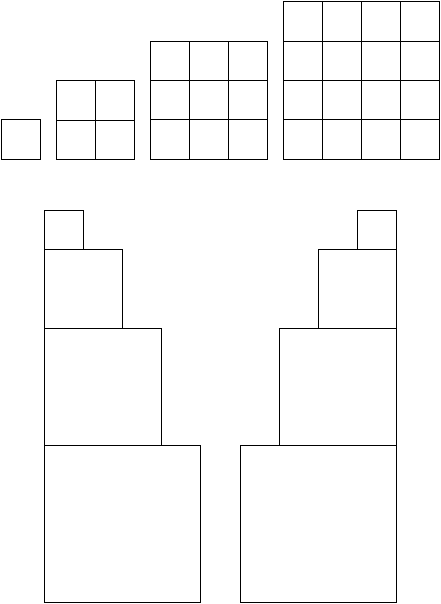
\includegraphics[scale=0.3]{FiguresMaths/SumSquares1}
\caption{The initial configuration for pictorially computing the sum of squares: the ``scaffolding".}
       \label{fig:sumSquares1}
\end{center}
\end{figure}
provides a schematic ``scaffolding" for the process:  The figure depicts two mirrored copies of the perfect squares $1^2$, $2^2$, $3^2$, and $4^2$ piled in decreasing order of size from bottom to top.  (To emphasize the pattern embodied by our procedure: the process of summing the first {\em five} perfect squares, $1^2$, $2^2$, $3^2$, $4^2$, $5^2$ would begin by just placing the $5 \times 5$ square array beneath the $4 \times 4$ array in Fig.~\ref{fig:sumSquares1}.)  The two piles are positioned in such a manner that there is:
\begin{itemize}
\item
a unit-width height-$(k=4)$ ``alley" between the $k \times k$ squares at the bottom of the ``scaffolding"
\item
a width-$3$ height-$(k-1)$ ``alley" between the $(k-1) \times (k-1)$ squares at the next lowest level of the ``scaffolding"
\item
a width-$5$ height-$(k-2)$ ``alley" between the $(k-2) \times (k-2)$ squares at the third lowest level of the ``scaffolding"

\hspace*{.5in}$\vdots$
\item
a width-$(2k-1)$ unit-height ``alley" between the two unit-side squares at the top level of the ``scaffolding"
\end{itemize}

\medskip

\noindent {\bf 2.}
Fig.~\ref{fig:sumSquares2}
\begin{figure}[htb]
\begin{center}
       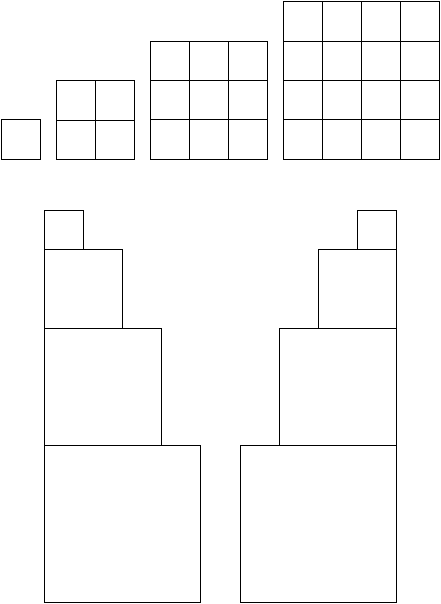
\includegraphics[scale=0.3]{FiguresMaths/SumSquares2}
\caption{Step 1 for pictorially computing the sum of squares: filling the unit-width ``alley" with the lower-lefthand unit-side squares.}
       \label{fig:sumSquares2}
\end{center}
\end{figure}
depicts the first rearrangement step.  The $(k=4)$ lower left unit-side squares are copied from their initial locations and moved to fill the height-$(k=4)$ ``alley" in the ``scaffolding".

\medskip

\noindent {\bf 3.}
Fig.~\ref{fig:sumSquares3}
\begin{figure}[htb]
\begin{center}
       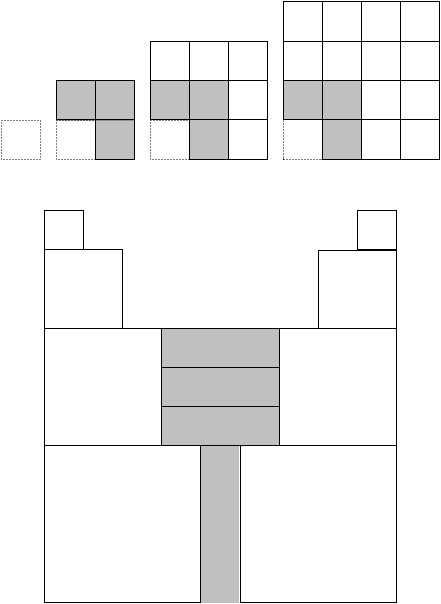
\includegraphics[scale=0.3]{FiguresMaths/SumSquares3}
\caption{Step 2 for pictorially computing the sum of squares: filling the width-$3$ ``alley" with the width-$3$
``bars" produced by flattening the length-$3$ L's.}
       \label{fig:sumSquares3}
\end{center}
\end{figure}
depicts the next step in the process.  From each perfect-square $k > 1$, we copy the $3$-square ``L-shape'' that sits atop the lower lefthand square.  We use the resulting length-$3$ ``bars" to fill in the width-$3$ ``alley" at the next lowest level in the ``scaffolding".

\medskip

\noindent \fbox{
\begin{minipage}{0.96\textwidth}
{\bf Explanatory note}.

The reader should recognize the kinship of the just-described process of taking L-shapes and flattening them into ``bars" with an analogous process in our pictorial proof of
Proposition~\ref{thm:squares-odd-integers-Gauss}.  In that proof, we represented each odd integer $2k+1$ as a length-$(2k+1)$ ``bar", and we bent the ``bar" into a reversed-L whose horizontal and vertical sub-``bars" each had length $k+1$.  In the current process, we are performing the exact inverse process---flattening instead of bending.
\end{minipage}
}

\bigskip

\noindent {\bf 4 and 5.}
Figs.~\ref{fig:sumSquares4} and~\ref{fig:sumSquares5}
\begin{figure}[ht]
\begin{center}
       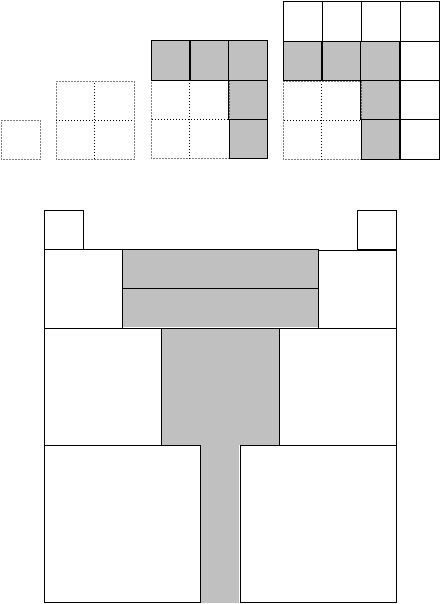
\includegraphics[scale=0.3]{FiguresMaths/SumSquares4}
\caption{Step 3 for pictorially computing the sum of squares: filling the width-$5$ ``alley" with the width-$5$ ``bars" produced by flattening the length-$5$ L-shapes.}
       \label{fig:sumSquares4}
\end{center}
\end{figure}
\begin{figure}[ht]
\begin{center}
       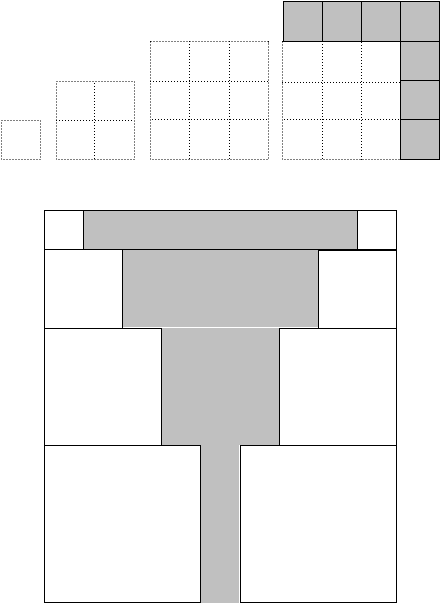
\includegraphics[scale=0.3]{FiguresMaths/SumSquares5}
\caption{Final step for pictorially computing the sum of squares: filling the width-$7$ ``alley" with the width-$7$ ``bars" produced by flattening the length-$7$ L-shapes.}
       \label{fig:sumSquares5}
\end{center}
\end{figure}
peel off successive-size L-shaped arrays from the adequately large initial square arrays, flatten these L's into ``bars", and use these ``bars" to fill in the next largest ``alley" in the scaffolding.

\medskip

We leave the detailed validation of the described process to the reader.

\paragraph{D. $\oplus$ Semi-pictorial solutions for $c=3$}

\index{Fubini, Guido} 
We described in Section~\ref{sec:summation-via-Fubini} how the Italian mathematician Guido Fubini was able to make notable mathematical progress by rearranging the representations of a variety of structured mathematical objects; see \cite{Fubini}.  Within the context of the current chapter, we apply such rearrangements to achieve exact values for some special subsums of $S_3(n)$, i.e., special sums of the cubes of integers.

\smallskip

The proof we develop here establishes relationships among three sets: the odd numbers $\{2i-1\}$, the perfect cubes $\{i^3\}$, and the triangular numbers $\{ \Delta_i \}$.  Specifically, we show that the sum of all odd numbers up to the triangular number $\Delta_k$ is equal to each of the following quantities:
\begin{itemize}
\item
the square of the triangular number $\Delta_k$
\item
the sum of perfect cubes up to $k$.
\end{itemize}
We provide pictorial reasoning that allows one to observe the equality between the preceding quantities.  Stated formally:

\begin{prop}
\label{thm:odds-sum2-cubes}
For all $k \in \N^+$,
\begin{equation}
\label{eq:sum-odds=Delta-sq=sum-cubes}
\Delta_k^2 \ \  = \ \
\sum_{i=1}^{\Delta_k} \ (2i-1)  \ \ =  \ \ \sum_{i=1}^k \ i^3
\end{equation}
\end{prop}

\begin{proof}
The lefthand equation in (\ref{eq:sum-odds=Delta-sq=sum-cubes}) follows from 
Proposition~\ref{thm:squares-odd-integers-Gauss}: the first $\Delta_k$ odd numbers sum
to $\Delta_k^2$.  We focus, therefore, only on the righthand equation.

\medskip

We take the odd integers in order and arrange them into groups whose successive sizes increase by $1$ at each step, as in the following triangular table (\ref{eq:triagular-table}).
\begin{equation}
\label{eq:triagular-table}
\begin{array}{llrrrrclcc}
\mbox{group $1$ (size $1$):} & &
1,  &    &     &      \\
\mbox{group $2$ (size $2$):} & &
3,  &  5, &     &      \\
\mbox{group $3$ (size $3$):} & &
7,  &  9, & 11, &     \\
\mbox{group $4$ (size $4$):} & &
13, & 15, & 17, & 19   \\
\vdots & & \vdots \\
\end{array}
\end{equation}
Group $1$ comprises just the smallest odd number, $1$; group $2$ comprises the next two odd numbers, $3$, $5$; group $3$ comprises the three odd numbers $7$,  $9$,  and $11$; and so on.  Let us observe some of the features of table (\ref{eq:triagular-table}).

We observe first that---at least within the illustrated portion of the table---the $i$ elements of the $i$th group add up to $i^3$:
\[
\begin{array}{llrrrrclcc}
\mbox{group $1$ (size $1$):} & &
1,  &    &     &     & \mbox{: sum} = &  1^3 \\
\mbox{group $2$ (size $2$):} & &
3,  &  5, &     &    & \mbox{: sum} =  &  2^3 \\
\mbox{group $3$ (size $3$):} & &
7,  &  9, & 11, &    &  \mbox{: sum} = &  3^3 \\
\mbox{group $4$ (size $4$):} & &
13, & 15, & 17, & 19 & \mbox{: sum} =  &  4^3 \\
\end{array}
\]

We observe next that, by construction, the $i$th group/row of odd integers in the table consists of the $i$ consecutive odd numbers beginning with the $\left( \Delta_{i-1} +1 \right)$th odd number, $2 \Delta_{i-1} +1$.  Since consecutive odd numbers differ by $2$, this means that the $i$th group (for $i>1$) comprises the following $i$ odd integers:
\[
2 \Delta_{i-1} +1, \ 2 \Delta_{i-1}  +3, \ 2 \Delta_{i-1}  +5 , \ \ldots, \ 2 \Delta_{i-1} + (2i-1)
\]
Therefore, invoking Proposition~\ref{thm:squares-odd-integers-Gauss}, the {\em sum} of the $i$ integers in group $i$, call it $\sigma_i$, equals
\begin{eqnarray*}
\sigma_i & = &
2 i \Delta_{i-1} \ + \ \big( 1 + 3 + \cdots + (2i-1) \big) \\
   & = & 2 i \Delta_{i-1} \ + \ \mbox{(the sum of the first $i$ odd numbers)} \\
   & = & 2 i \Delta_{i-1} \ + \ i^2
\end{eqnarray*}
By direct calculation, then, 
\[ \sigma_i \ \ = \ \ 2i  \cdot \frac{i(i-1)}{2} \ + \ i^2 \ \ = \ \
(i^3 - i^2)  \ + \ i^2 \ \ = \ \ i^3
\]

\noindent
The proof is now completed by concatenating the rows of table (\ref{eq:triagular-table}) and
observing the pattern that emerges:
\[ (1) \ + \ (3 + 5) \ + \ (7 + 9 + 11) \  + \cdots
\ \ = \ \ 1^3 \ + \ 2^3 \ + \ 3^3 \ + \cdots 
\]
Note the ``Fubini-esque" arrangements and groupings throughout this argument. (To understand this reference, see Fubini's role in Section~\ref{sec:summation-via-Fubini}.)  \qed
\end{proof}

\ignore{************
You should now verify by induction that $2 \Delta_{i-1} +(2i-1) \ = \ 2 \Delta_{i} -1$, 
which gives us another expression for the last odd integer in group $i$.  
Once one verifies that $2 \Delta_{i-1} +2i-1 \ = \ 2
\Delta_{i} +1$, one discovers that this group has the sum
{\Denis Induction is not needed, the expression is simply obtained by definition of triangular numbers.}
\[
2i \Delta_{i-1}  \ - \ 2 \Delta_{i-1} +i  \  = \
(2i -1) \Delta_i + i \ = \ i^3.
\]

In other words, group $i$ consists of the odd numbers
\[ 2 \Delta_{i-1} +1, \ 2 \Delta_{i-1} +3, \  \ldots, \  2\Delta_i -1 \]
**************}

We now present a {\em pictorial} proof of a portion of Proposition~\ref{thm:odds-sum2-cubes}, namely, the relation between sums of perfect cubes  and squares of triangular numbers.  This illustration provides a {\em non-textual} way to understand this result, and---at least as importantly---it provides a fertile setting for seeking other facts of this type.

\begin{prop}
\label{thm:cubes-sumto-Delta-saquared}
For all $k \in \N^+$,
\[ 1^3 \ + \ 2^3 \ + \cdots + \ k^3 \ \ = \ \ \Delta_k^2 \]
\end{prop}

\begin{proof}
We develop an induction that reflects the structure of Table (\ref{eq:triagular-table}).

\smallskip

\noindent {\sf Base cases.}
The base of our induction is the first case of the claimed result:
\[  1^3 \  = \ 1 \ = \ \Delta_1^2 \]

While this first (and obvious) case is enough for the induction, it does not tell us much about the structure of the problem.  Therefore, we consider also the next step, namely, the case $k=2$:
\[  1^3 + 2^3 \ = \ 9 \ = \ \Delta_2^2 \]
We depict in Fig.~\ref{fig:sumCubes1} how to obtain a ``larger" base case for our induction by pictorially summing the numbers from the first two groups in Table (\ref{eq:triagular-table}).
\begin{figure}[hbt]
\begin{center}
       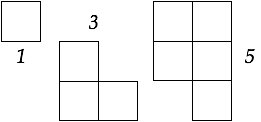
\includegraphics[scale=0.35]{FiguresMaths/SumCubes1} \hspace{2cm}
       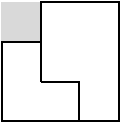
\includegraphics[scale=0.35]{FiguresMaths/SumCubes1bis}
\caption{(Left) Pictorially depicting the first two groups from Table (\ref{eq:triagular-table}) as stacked unit-side squares: the set $\{1\}$ of group $1$ and the set $\{3, 5\}$ of group $2$. (Right) Illustrating how to form a $3 \times 3$ square by pictorially summing the numbers $1$, $3$, and $5$.  The clear portions of the square come from  group $2$; the shaded small square at the top comes from group $1$.}
       \label{fig:sumCubes1}
\end{center}
\end{figure}
Observe that we can fit the shapes from the left side of the figure together to form the $\Delta_2 \times \Delta_2$ square.

\medskip

\noindent {\sf Inductive hypothesis}.
Say for the sake of the induction that the target equality holds for all $i < k$; i.e.,
\[ 1^3 \ + \ 2^3 \ + \cdots + \ i^3 \ \ = \ \ \Delta_i^2 \ \ = \ \ {{i+1} \choose 2}^2 \]

\medskip

If we go one step further, to incorporate group $3$, i.e., the set $\{7, 9, 11\}$, into our pictorial summation process, then we discover that mimicking the process of Fig.~\ref{fig:sumCubes1} is a bit more complicated for this case.  A bit of analysis exposes that the more complicated manipulation required to form the $\Delta_3 \times \Delta_3$ square is a consequence of the odd cardinality of the group-$3$ set.  Accordingly, we must extend our induction in slightly different ways for the cases of odd and even $k$.

\medskip

\noindent {\sf Inductive extension for odd $k$}.
In order to extend the induction hypothesis in this case, we need to prove that
\[ \Delta_k^2 \ \ = \ \ \Delta_{k-1}^2 \ + \ k^3 \]
We begin to garner intuition for this extension by comparing the quantities $\Delta_k^2$ and $1 + 2^3 + \cdots + k^3$.

\smallskip

Moving to the pictorial domain, we write $k^3$ as $k \times k^2$, and we distribute $k \times k$ square blocks around the $\Delta_{k-1} \times \Delta_{k-1}$ square, as shown in Fig.~\ref{fig:sumCubes3} for the case $k=3$. 
\begin{figure}[ht]
\begin{center}
       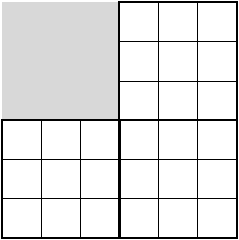
\includegraphics[scale=0.35]{FiguresMaths/SumCubes3}
\caption{Extending the inductive summation-by-manipulation for the case of odd $k$:  The manipulation of small squares produces the next bigger perfect square.  (The case $k=3$ is depicted.)}
       \label{fig:sumCubes3}
\end{center}
\end{figure}
Because $k$ is odd, the small squares pack perfectly---since $(k-1)$ is even, hence divisible by $2$.   The depicted case depicts pictorially the definition of triangular numbers: $k \cdot \frac{1}{2}(k-1) \ = \ \Delta_{k-1}$.

\medskip

\noindent {\sf Inductive extension for even $k$}.
The basic reasoning here mirrors that for odd $k$, with one small, but major difference.   Now,  as we assemble small squares around the large square, two subsquares overlap, as depicted in Fig.~\ref{fig:sumCubesEven}.
\begin{figure}[hbt]
\begin{center}
       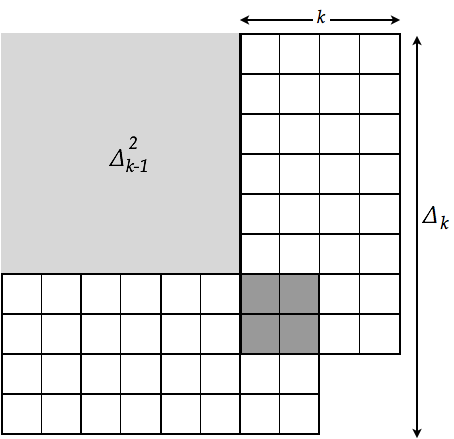
\includegraphics[scale=0.35]{FiguresMaths/SumCubesEven}
\caption{The construction for even $k$ produces  an overlapped area represented in dark grey (the figure depicts the case $k=4$).}
       \label{fig:sumCubesEven}
\end{center}
\end{figure}
We must manipulate the overlapped region in the manner depicted in Fig.~\ref{fig:sumCubesEvenFinal} in order to get a tight packing around the large square.
\begin{figure}[hbt]
\begin{center}
       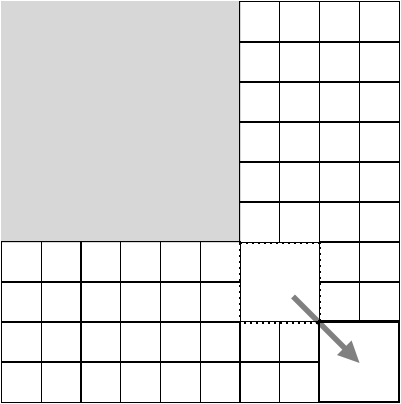
\includegraphics[scale=0.35]{FiguresMaths/SumCubesEvenFinal}
\caption{How to obtain a large ($\Delta_k \times \Delta_k$) square by sliding the overlapped small square region into the like-sized small square empty region.}
       \label{fig:sumCubesEvenFinal}
\end{center}
\end{figure}
Happily, when there is a small overlapping square region, there is also an identically shaped empty square region, as suggested by these two figures.  We provide a bit more detail.  Because $(k-2)$ is even, the like-configured square blocks can be allocated to two sides of the initial $\Delta_{k-1} \times \Delta_{k-1}$ square---namely, its right side and its bottom---in the manner depicted in Fig.~\ref{fig:sumCubesEven}.  One can discern in the figure the overlap we described: it has the shape of a square that measures  ${1 \over 2} \left( \Delta_k - \Delta_{k-1}\right)$ on a side.  One also sees in the figure an empty square in the extreme bottom right of the composite $\Delta_k \times \Delta_k$ square, which matches the overlapped square identically.  This situation is the pictorial version of the equation
\[ \Delta_k^2 \ - \ \Delta_{k-1}^2 
 \ \ =  \ \ {1 \over 4} k^2 \left( (k+1)^2 - (k-1)^2 \right)  \ \ = \ \ k^3 \]

We have thus extended the inductive hypothesis for both odd and even $k$, whence the
result.  \qed
\end{proof}


\subsubsection{$S_c(n)$ for general {\em negative} $c$th powers}
\label{sec:sum-of-i2c<0}

We focus finally on summations of the form
\[ S_c(n) \ \eqdef \ \sum_{i=1}^n \ i^c \]
for arbitrary {\em negative} numbers $c$.  The reader can garner intuition for the upcoming bounds from the general shape of the rectangles and continuous curves in Figs.~\ref{fig:riemann-harmonic1} and~\ref{fig:riemann-harmonic2}.

\begin{prop}
\label{thm:general-bounds-negative-xc}
For summations $S_c(n)$ with fixed negative powers $c<0$,
\begin{equation} 
\label{eq:general-bounds-negative-xc}
\left[
\underline{C}_c(n) \ = \ \int_0^{n-1} \ (x+1)^c dx
\right]
\ \leq \ S_c(n) \ \leq \
\left[
\overline{C}_c(n) \ = \ \int_1^n \ x^c dx
\right]
\end{equation}
\end{prop}

\begin{proof}
We obtain our upper bound on the sum of $S_c(n)$ by evaluating the integral that yields the area $\overline{C}_c(n)$ under the righthand continuous curve ($a$) in the analogue of Fig.~\ref{fig:riemann-harmonic1} for $S_c(n)$.  We obtain our lower bound on $S_c(n)$ by evaluating the integral that yields the area $\underline{C}_c(n)$ under the lefthand continuous curve ($b$) in the analogue of Fig.~\ref{fig:riemann-harmonic2} for $S_c(n)$.  \qed
\end{proof}

When $c \neq -1$,\footnote{We need to avoid the case $c = -1$ so that we do not attempt to divide by $0$.}~we can provide more detail, by using reasoning similar to that underlying the bounds (\ref{eq:bounds-sum-xc}) that hold for positive values of $c$.

\paragraph{A. Negative powers $-1 < c < 0$}

In this case, we obtain essentially the same bounds as in the case of nonnegative $c$.  To wit:

\begin{prop}
\label{thm:bounds-(-1)<c<0}
For summations $S_c(n)$ with fixed negative powers in the range $-1 < c<0$,
\begin{equation}
\label{eq:bounds-(-1)<c<0}
\begin{array}{l}
\mbox{For $-1 < c< 0$:} \\
 \\
\hspace*{.35in}
{\displaystyle \frac{1}{c+1} n^{c+1} \ - \ O(n^c)}
  \ \ \leq \ \ S_c(n)
  \ \ \leq \ \
{\displaystyle \frac{1}{c+1} n^{c+1} \ + \ O(1)}
\end{array}
\end{equation}
The infinite version of summation $S_c(n)$, namely, the series
$\displaystyle S_c^{(\infty)} \ \eqdef \ \sum_{i=0}^\infty i^c$,
diverges.
\end{prop}

We thus observe that $S_c(n)$ has the same growth {\em pattern} with increasing $n$ as it does when $c$ is positive, but that $S_c(n)$'s growth {\em rate} is slower because of the damping effect the negative $c$ in the exponent.  This damped growth notwithstanding, the infinite series $S_c^{(\infty)}$ diverges because $n^{c+1}$, which is the variable portion of the lower bound on $S_c(n)$, grows without bound as $n$ grows without bound.

\paragraph{B. Negative powers $c < -1$}

When $c$ is ``very negative'', specifically, when $c < -1$, the infinite version of $S_c(n)$, call it $S_c^{(\infty)}$, is a {\em convergent} infinite series.  In this case, $n^c$ {\em shrinks} as $n$ grows, so an analysis mirroring the one that leads to (\ref{eq:bounds-(-1)<c<0}) provides the following sum for $S_c^{(\infty)}$.

\begin{prop}
\label{thm:bounds-negative-(not-1)-sum-xc}
When the fixed negative power $c$ is smaller than $-1$, then the
infinite version, $S_c^{(\infty)}$, of $S_c(n)$, converges, with the
following sum.
\begin{equation}
\label{eq:bounds-negative-(not-1)-sum-xc}
S_c^{(\infty)} \ = \ \frac{1}{c+1}
\end{equation}
\end{prop}

\begin{proof}
We see as in (\ref{eq:bounds-(-1)<c<0}) that, for $c<-1$, as $n$ grows without bound, $S_c(n)$ tends to the value ${\displaystyle \frac{1}{c+1}}$.  \qed
\end{proof}

\paragraph{C. Negative powers $c = -1$: the {\em harmonic} series}

\index{harmonic series $S^{(H)}$}
The singular case defined by the value $c = -1$ defines the important {\it harmonic series},
\[ S^{(H)} \ = \ \sum_{i=1}^\infty \ \frac{1}{i} \]
and its finite prefixes that comprise the {\it harmonic summation}
\[ S^{(H)}(n) \ = \ \sum_{i=1}^n \ \frac{1}{i} \]
\index{harmonic summation $S^{(H)}(n)$}

\smallskip

\index{harmonic summation $S^{(H)}(n)$!asymptotic behavior} \index{Euler, Leonhard}
\index{Napier, John} \index{Euler's constant}
{\it (i) The asymptotic behavior of $S^{(H)}(n)$.}
It has been known since the time of the well-traveled Swiss mathematician Leonhard Euler that $S^{(H)}$ and $S^{(H)}(n)$ are closely related to the {\em natural}, or, {\it Napierian}\footnote{The natural logarithm, i.e., the logarithm to the base $e$, is commonly referred to as the {\it Napierian logarithm}, in honor of the Scottish polymath John Napier.}~logarithm $\ln n$, i.e., the logarithm whose base is Euler's constant $e = 2.718281828 \ldots$.

\begin{prop}
\label{thm:harmonic}
The behavior of the harmonic summation $S^{(H)}(n)$ as a function of $n$ is given by
\[ S^{(H)}(n) \ \approx \ \ln n \]
It follows, in particular, that the harmonic series $S^{(H)}$ diverges.
\end{prop}

\bigskip

\noindent \fbox{
\begin{minipage}{0.96\textwidth}
{\bf Enrichment note}.

\index{harmonic series  $S^{(H)}$!relation to music}
The adjective ``harmonic'' calls to mind a number of concepts associated with {\em music}, such as ``harmonics'' and ``harmony''.  The association between our series and these musical concepts is not a coincidence.  The name of the harmonic series derives from the concept of {\em overtones}, or {\em harmonics}, in music.  When one observes a vibrating string, one finds that the wavelengths of its overtones, as fractions of the string's fundamental wavelength, are the terms of the {\em harmonic sequence}, namely, $\frac{1}{2}$, $\frac{1}{3}$, $\frac{1}{4}$, \ldots.  
\end{minipage}
}
\bigskip

%{\Denis I developed a graphical way to interpret the harmonic sum and its link with the neperian log (this is I believe very interesting and original.
%May be this is the wrong place, tell me (we can also split the
%following into smaller pieces...)}

\index{harmonic summation $S^{(H)}(n)$!understanding logarithmic behavior}
{\it (ii) Bounds on the asymptotic behavior of $S^{(H)}(n)$.}
Fig~\ref{fig:HarmonicSumInitial} depicts the harmonic summation $S^{(H)}(n)$ as the area of abutting unit-width rectangles of respective heights (from left to right) of $1$, $1/2$, $1/3$, \ldots, $1/n$.
\begin{figure}[htb]
\centerline{
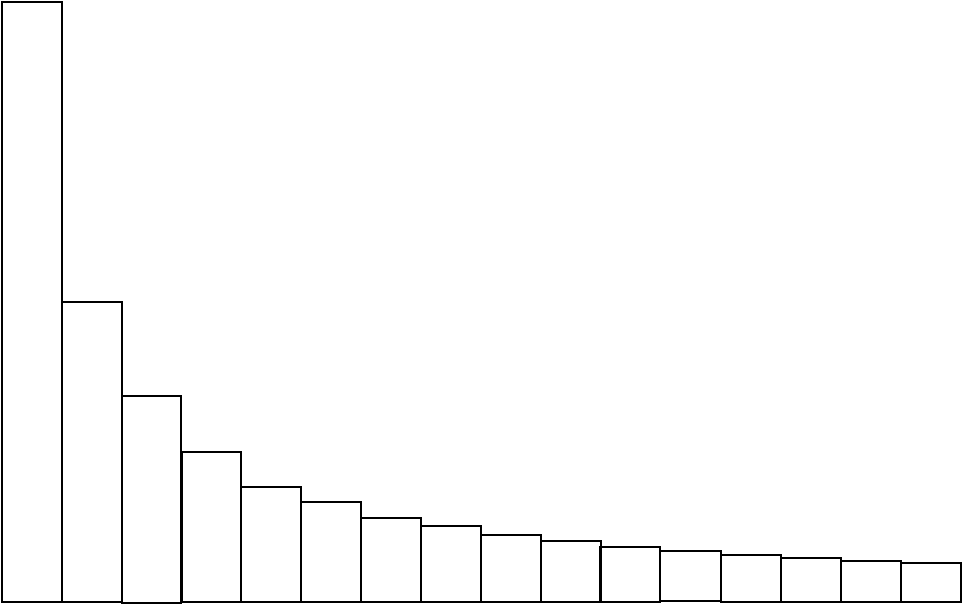
\includegraphics[scale=0.2]{FiguresMaths/HarmonicSumInitial}
}
\caption{The harmonic summation $S^{(H)}(n)$ represented by the area of abutting unit-width rectangles whose (decreasing) heights form the sequence of consecutive integer reciprocals.}
\label{fig:HarmonicSumInitial}
\end{figure}

\medskip

We now reorganize the sequence of $S^{(H)}(n)$'s summands in a way that helps us better understand the behavior of $S^{(H)}(n)$ as a function of $n$.
\begin{itemize}
\item
We group $S^{(H)}(n)$'s summands into sub-summations whose sizes are the consecutive powers of $2$:
\[ \begin{array}{llcl}
\mbox{The first $(2^0 =1)$ reciprocal:} &
A_0 & = &  {\displaystyle 1 } \\[1.01em]
\mbox{the next $(2^1 =2)$ consecutive reciprocals:} &
A_1 & = &  {\displaystyle \frac{1}{2} + \frac{1}{3} }  \\[1.01em]
\mbox{the next $(2^2 =4)$ consecutive reciprocals:} &
A_2 & = &  {\displaystyle \frac{1}{4} + \frac{1}{5} + \frac{1}{6} + \frac{1}{7} } \\
\vdots &  & & \vdots \\
\mbox{the next $2^i$ consecutive reciprocals:} &
A_i & = &  {\displaystyle \frac{1}{2^i} + \frac{1}{2^i+1} + \cdots +
     \frac{1}{2^{i+1}-1}  } \\
\vdots &  & & \vdots \\
\end{array}
\]
\item
We derive constant upper and lower bounds for each subsum.  Focus on the $2^i$ consecutive reciprocals of the generic subsum $A_i$.  The largest of these reciprocals is $1/2^i$; the smallest is $1/(2^{i+1}-1)$.  We therefore note that
\[
\frac{1}{2}
 \ < \
\frac{2^i}{2^{i+1}-1}
 \ < \
2^i \cdot A_i
  \ < \
\frac{2^i}{2^i}
  \ = \ 1
\]

In summary: each subsum $A_i$ lies strictly between $2^{-i-1}$ and $2^{-1}$.
\end{itemize}

We can interpret our bounds on the subsums $A_i$ in the light of Fig.~\ref{fig:HarmonicSumInitial}.   Let us proceed left to right along the abutting rectangles in the figure, and let us recall, from Section~\ref{sec:exponential-function}, the definition of
``logarithm to the base $b$''.  As we double the number of rectangles that we have traversed, consider the increase in the aggregate area of the thus-far traversed rectangles:
\begin{enumerate}
\item
{\em This increase is no larger than} $1$.

\smallskip

This means that {\em $S^{(H)}(n)$ grows no faster than $\log_2 n$.}

\item
{\em This increase is greater than} $1/2$.

\smallskip

This means that {\em $S^{(H)}(n)$ grows faster than $\log_4 n$.}
\end{enumerate}
Of course, these observations are consistent with the verified actual natural-logarithmic growth rate of $S^{(H)}(n)$, because $2 < e < 4$.

\begin{figure}[htb]
\centerline{
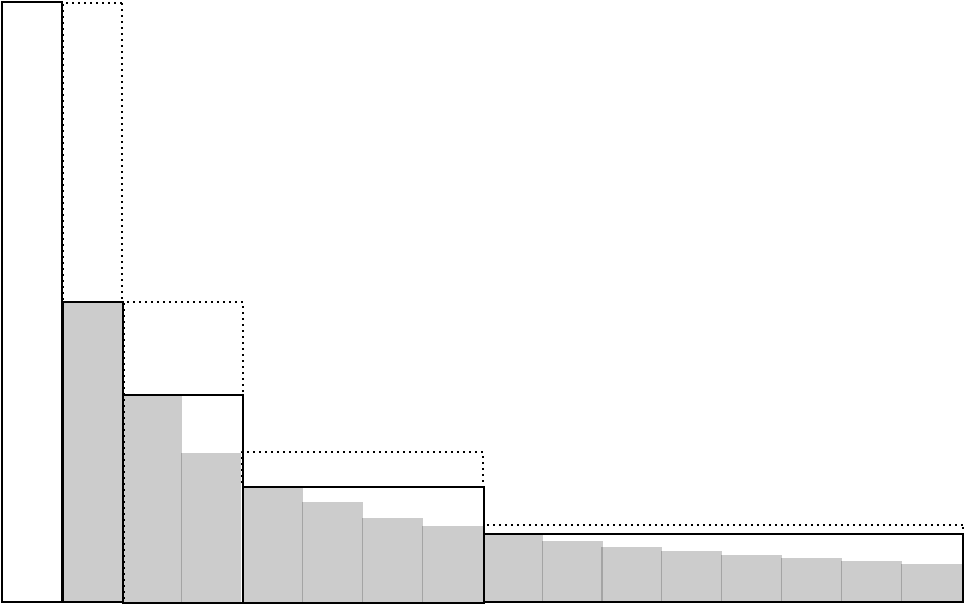
\includegraphics[scale=0.24]{FiguresMaths/HarmonicSumUpperbound}
}
\caption{Upper-bounding $A_i$ by larger unit-size rectangles in the harmonic sum.}
\label{fig:HarmonicSumUpperbound}
\end{figure}

\begin{figure}[htb]
\centerline{
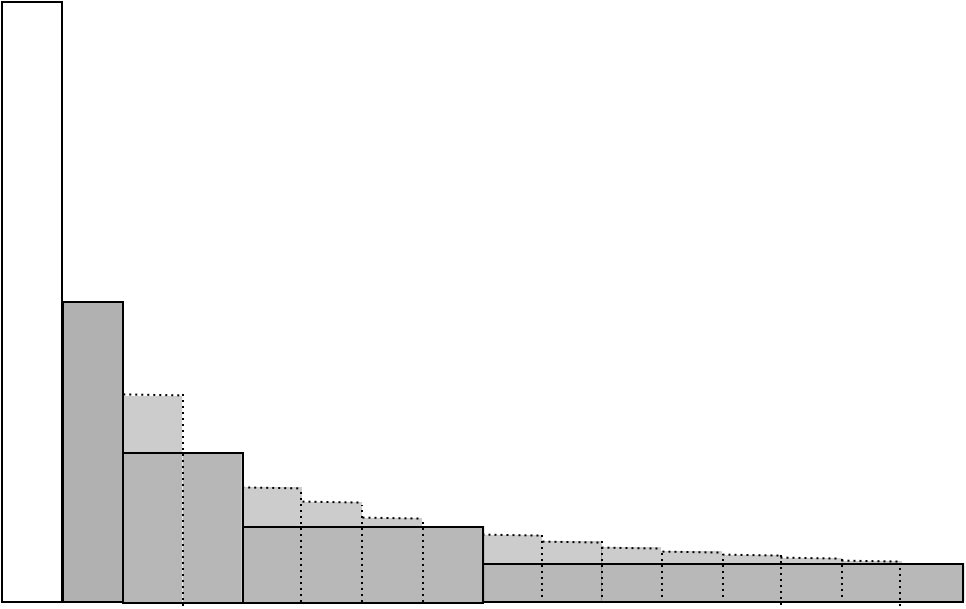
\includegraphics[scale=0.24]{FiguresMaths/HarmonicSumLowerbound}
}
\caption{A pictorial lower bound for the harmonic summation.}
\label{fig:HarmonicSumLowerbound}
\end{figure}



%%%%%%%%%%%%%%%%%%%%%%%%%%%%%%%%%%%%%%%%%%%%%%%%

\section{Exercises: Chapter 6}

Throughout the text, we mark each exercise with 0 or 1 or 2 occurrences of the symbol $\oplus$, as a rough gauge of its level of challenge.  The 0-$\oplus$ exercises should be accessible by just reviewing the text.  We provide {\em hints} for the 1-$\oplus$ exercises; Chapter~\ref{ch:Exercises} provides {\em solutions} for the 2-$\oplus$ exercises.  Additionally, we begin each exercise with a brief explanation of its anticipated value to the reader.

\begin{enumerate}
\item
{\bf A ``pictorial" summation of the first $n$ integers}

{\sc Lesson:} A practice solo ride toward a simple ``pictorial" argument

\smallskip

{\em Flesh out the use of Fig.~\ref{fig:anotherSumOdds} and its following text to produce a rigorous derivation of the formula for the sum of the first $n$ integers.}
\smallskip

\item
{\bf A ``pictorial" summation of $S^{(\infty)}_{1/2}$}

{\sc Lesson:} Another practice solo ride toward a simple ``pictorial" argument

\smallskip

{\em Derive the sum of $S^{(\infty)}_{1/2}$ by developing the pie-slicing argument of Fig.~\ref{fig:sumGeo1sur2circle} and its accompanying text.}

\smallskip

\item
{\bf Solving summation $S_b^{(2)}(n)$ algebraically}

{\sc Lesson:} A practice solo ride which expands a complicated inductive argument by one step

\smallskip

{\em Build on the proof of Proposition~\ref{thm:sum-i2i} to solve summation $S_b^{(2)}(n)$.}
\medskip

\item
{\bf Evaluating $S_1(n) = \sum_{i=1}^n \ i$, using the fact that $S_2(n) = \sum_{i=1}^n \ i^2$}

{\sc Lesson:} Practice in manipulating mathematical expressions

\smallskip

Say that someone gives you a machine that can compute the summation of the first $n$ perfect squares, given $n$ as an input:
\[ S_2(n)  \ = \ 1 \  + \ 4 \ + \ 9 \ +  \cdots + \ n^2 \]

{\em Show how to use this machine in order to compute the sum of the first $n$ integers.}

\smallskip

{\em Hint.}
Try to think creatively.  Think of how one can (mathematically) relate the first $n$ integers to their squares.
\medskip

\item
{\bf Evaluating $S_2(n) = \sum_{k=1}^n \ k^2$, given knowledge that $S_2(n) = \Theta(n^3)$}

{\sc Lesson:} Practice with solving systems of $n$ linear equations in $n$ unknowns, applied to the {\it method of undetermined coefficients}

\index{method of undetermined coefficients}

\smallskip

Say that you know---perhaps from reading Section~\ref{sec:riemann-bounds}---that the sum of the first $n$ perfect squares is a {\em cubic} polynomial in $n$.

\smallskip

{\em Use the method of undetermined coefficients to derive the exact formula (\ref{eq:sum-1-to-nsq1}) for the sum.}

\medskip
\item
$\oplus$
{\bf Evaluating a geometric summation pictorially}

{\sc Lesson:} Experience using pictorial representations

\smallskip

In Section~\ref{sec:summing-geometric-series:techniques}, we used Thales's theorem about similarity in triangles (Theorem~\ref{thm:Thm-of-Thales-similarity}) to sum the simple infinite geometric series $\sum_{i=0}^\infty \ b^i$.  It turns out that a modest modification of that evaluation strategy allows us also to evaluate the truncated versions of that series, namely, the summations
\[ S^{(b)}(n) \ = \ \sum_{i=0}^n \ b^i \]

{\em Use the following figure to evaluate $S^{(b)}(n)$.}

\centerline{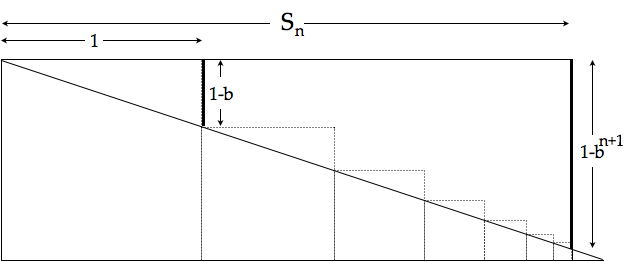
\includegraphics[scale=0.4]{FiguresArithmetic/ThalesGeometricSumFinite}}


\bigskip
\item
{\bf A direct proof that the harmonic series diverges}
\index{harmonic series}

{\sc Lesson:}
Practice with manipulating summations and series

\smallskip

There are myriad ways to prove that the harmonic series
\[ S^{(H)} \ = \ \sum_{k=1}^\infty \ {1 \over k} \]
diverges.  In Proposition~\ref{thm:harmonic}, we developed a method that provided additional information: not only did it prove that $S^{(H)}$ diverges---i.e., tends to infinity as one looks at more and more terms grows---it also exposed the rate of this divergence as logarithmic in the number of terms one looks at.  If one wants only to prove divergence, then the following more direct argument will suffice.

\medskip

{\em Develop a proof that the harmonic series diverges by
\begin{itemize}
\item
partitioning $S^{(H)}$'s terms into groups whose sizes are successive powers of $2$
\item
developing an argument based on the sums within the groups.
\end{itemize}
}

\smallskip

{\em For clarification:}
The partitioning step operates as follows:
{\footnotesize
\[ 
\begin{array}{ll}
S^{(H)} 
             & = \ 1 \ + \ {1 \over 2} + {1 \over 3} + {1 \over 4} + {1 \over 5} + {1 \over 6}+ {1 \over 7} + {1 \over 8} + {1 \over 9} + {1 \over 10}+ {1 \over 11}  +{1 \over 12} + {1 \over 13} + {1 \over 14}+ {1 \over 15} + \cdots \\
             & \\
  & = \ (1)  +  \left( {1 \over 2} + {1 \over 3} \right)  +  \left( {1 \over 4} + {1 \over 5} + {1 \over 6}+ {1 \over 7} \right)  +  \left( {1 \over 8} + {1 \over 9} + {1 \over 10}+ {1 \over 11}  +{1 \over 12} + {1 \over 13} + {1 \over 14}+ {1 \over 15} \right) \ +\cdots
\end{array} \]
}

\item
$\oplus$ {\bf Summations, and summations of summations}

{\sc Lesson:} Practice manipulating summations; gain familiarity with basic sums

\smallskip

By definition:
\[ Id_n \ \eqdef \ \sum_{k=1}^n \ 1 \ = \ 1 + 1 + \cdots +1 \  = \ n \]

We have proved in multiple ways:
\[ \Delta_n \ \eqdef \  \sum_{k=1}^n \ k \ = \ 1+2+3+ \cdots +n \ = \ \frac{1}{2} Id_n \cdot (n+1) \]

\smallskip

This exercise picks up where these two examples leave off.

  \begin{enumerate}
  \item 
{\em Prove that}\footnote{The sum of the the first $n$ triangular numbers, $\sum_{k=1}^n \ \Delta_k$, is often denoted $\Theta_n$.  We employ instead the nonstandard name $\widehat{T}_n$ to ensure that we do not confuse the newcomer who has recently learned about the role of the letter $\Theta$ in asymptotic notation.} 
\[ \widehat{T}_n \ \eqdef \  \sum_{k=1}^n \ \Delta_k \ = \   
\Delta_1 + \Delta_2 + \cdots + \Delta_n \ = \ \frac{1}{3} \Delta_n \cdot (n+2) \]

  \item
$\oplus \oplus$
{\em Develop and verify a formula for the summation:}
\[ \Upsilon_n  \ \eqdef \  \sum_{k=1}^n \ \widehat{T}_k \ = \  
\widehat{T}_1 + \widehat{T}_2 + \cdots + \widehat{T}_n \]

  \item
{\em Prove the following identities involving $\Delta_n$.  For all $n \in \N^+$:}
    \begin{enumerate}
    \item
$\Delta_n \ + \ \Delta_{n-1} \ = \ n^2$

\smallskip

This is a straightforward exercise in algebraic manipulation.  Can you {\em also} find an ``interesting" proof of this identity, say one that employs a ``pictorial" representation of $\Delta_n$?

    \item
$\Delta_n^2 \ - \ \Delta_{n-1}^2 \ = \ n^3$

\smallskip

{\em Hint}: Try ``playing" with simple manipulations of the equation 
\[ \Delta_n \ = \ n \ + \ \Delta_{n-1} \]
which defines $\Delta_n$.
   \end{enumerate}

  \item
$\oplus$
{\em Derive a closed-form expression for the sum}
\[ \widehat{T}_n \ + \ \widehat{T} _{n-1} \]

\smallskip

{\em Hint}: Recall that the sums $\widehat{T}_i$ are defined as sums of $\Delta_j$, which, in turn, are defined by closed-form expressions.  Lots to ``play" with!
  \end{enumerate} 
\end{enumerate}

\ignore{****************
\subsection{Sum of perfect cubes}

\noindent \textit{The aim.}
Presenting an alternative proof of the result of Section~\ref{sec:sumOfOdds},
that establishes that the sum of $n$ first cubes is equal to a perfect square.
\medskip

\noindent \textit{The problem.}
Show that the sum of the $n$ first cubes is equal to a perfect square, and more precisely, $\Delta_n^2$.
\medskip

\noindent \textit{Hint.}
Use the the simple pattern of multiplication tables that we learned in elementary school.
\medskip

\noindent \textit{Learning lessons.}
Show an alternative proof. 
***********************}


\ignore{**************
%and more generally, $A_i$ is the sum of the consecutive $\frac{1}{i}$
%(for $k$ such that $\frac{1}{2^i+1} \leq k \leq \frac{1}{2^{i+1}}$). 
Note that each $A_i$ is the sum of $2^i$ consecutive terms.

We claim that each partial sum satisfies $A_i \leq 1$.  Verifying this
by actually summing each $A_i$ requires a bit of calculation, but if
we want only the bound, then we achieve that quite easily from the
drawing in Fig~\ref{fig:HarmonicSumUpperbound}.
\begin{figure}[htb]
\centerline{
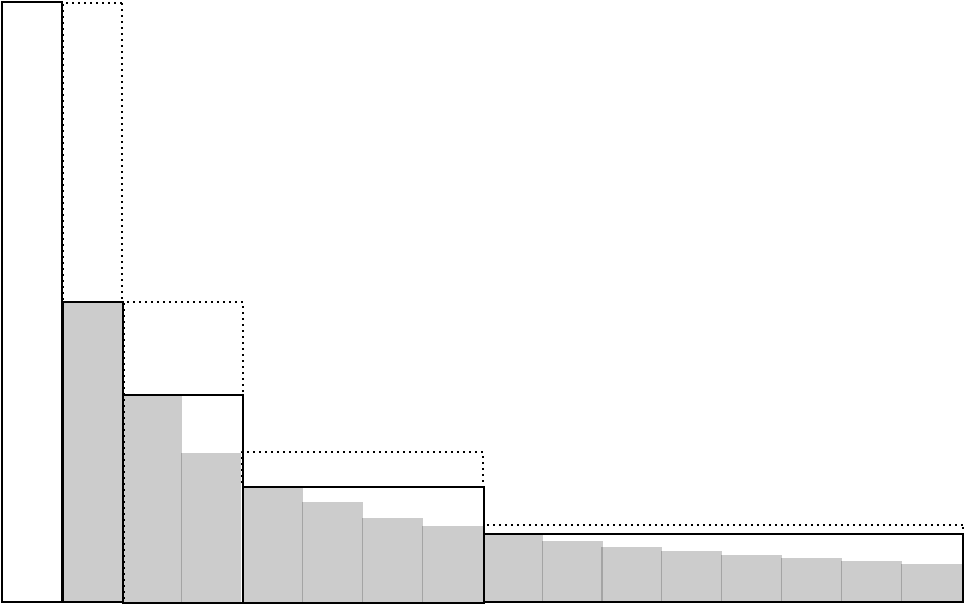
\includegraphics[scale=0.3]{FiguresMaths/HarmonicSumUpperbound}
}
\caption{Upper bound of $A_i$ by larger unit-size rectangles in the harmonic sum.}
\label{fig:HarmonicSumUpperbound}
\end{figure}

constant value $k$.  This claim is verified with the value $k=1$ by
the drawing in Fig~\ref{fig:HarmonicSumUpperbound}. shows that all the
$A_i$ are lower than $1$ but we could have considered a more accurate
value, however, it is enough and simple.  This result is obtained by
embedding each term $A_i$ by larger rectangles (of unit surfaces), the
upper bound is the bold rectangle plus the dashed rectangle at the
top.  {\Denis I hope my previous explanation is clear enough...}


Going into more detail, we claim that the partial sums $A_i$ form an
increasing sequence.  Here again, an exact verification by calculating
each $A_i$ is onerous to achieve, but the claim can be verified
graphically from the drawing in Fig~\ref{fig:HarmonicSumLowerbound}.
\begin{figure}[htb]
\centerline{
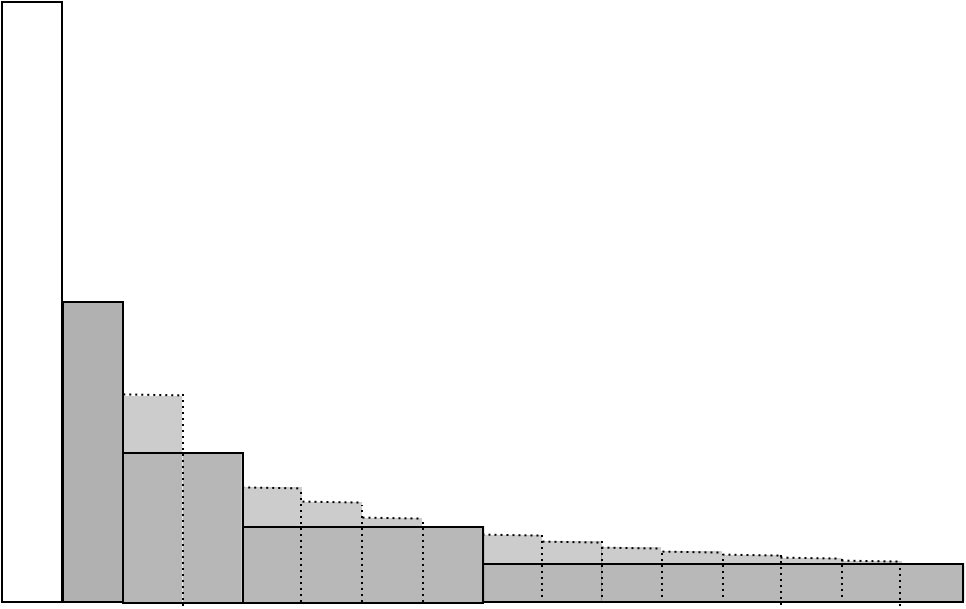
\includegraphics[scale=0.3]{FiguresMaths/HarmonicSumLowerbound}
}
\caption{A pictorial lower bound for the harmonic summation.}
\label{fig:HarmonicSumLowerbound}
\end{figure}
The drawing suggests the following exact sequence of analyses.

Let us verify first that $A_2 \geq A_1$ by showing that $A_2-A_1 \geq
0$; this inequality corresponds to the leftmost light grey rectangle
in Fig~\ref{fig:HarmonicSumLowerbound}.  We want to sum
\[ A_2-A_1 \ = \ \frac{1}{5} + \frac{1}{6} + \frac{1}{7} + \frac{1}{8}
- \frac{1}{3} - \frac{1}{4} \]
Because $\displaystyle \frac{1}{5} \geq \frac{1}{6}$ and
$\displaystyle \frac{1}{7} \geq \frac{1}{8}$, we have
\[
A_2-A_1 \ \ \geq \ \
\left(\frac{1}{6} + \frac{1}{6}\right) - \frac{1}{3} +
\left(\frac{1}{8} + \frac{1}{8}\right) - \frac{1}{4}
  \ \ =  \ \  0.
\]
Hence, $A_2 \geq A_1$. 

We continue to use such grouped calculations to prove that each
$A_{i+1} \geq A_i$.  To wit, we group $\displaystyle \frac{1}{2^{i+1}
  + 1} + \frac{1}{2^{i+1} + 2}$ with $\displaystyle -\frac{1}{2^{i} +
  1}$.  Because $\displaystyle \frac{1}{2^{i+1} + 1} \geq
\frac{1}{2^{i+1} + 2}$, we have $\displaystyle \frac{1}{2^{i+1} + 1} +
\frac{1}{2^{i+1} + 2} - \frac{1}{2^{i} + 1} \geq 0$.  We conclude that
$A_{i+1} \geq A_i$.

Finally, as the sequence $A_i$ is bounded above and increasing, it converges to a constant.


The preceding grouping of the terms of $S^{(H)}(n)$, combined with our
bounds on the generic $A_i$


coupled with the
the fact that
The explanation relies on the following observations of the harmonic series:
$S^{H}(2^{i+1}-1) = S^{H}(2^{i}-1) + A_i$

From a given value of $i$, each $A_i$ and its successive values have roughly the same value equal to the limit of $A_i$.
In other words, we go from index $2^i$ to $2^{i+1}$ in $S^{H}$ by a multiplication by $2$ that corresponds to adding a constant. 
This is exactly what the log means!
***************}

\ignore{***************

\noindent \textit{The aim.}
$\Theta_n$ is defined as the sum of the triangular numbers $\Delta_n$:

$\Theta_n =  \sum_{k=1}^{n} \Delta_k$

Our goal here is to give an expression of these numbers.
\medskip

\noindent \textit{The problem.}
Prove the following expression by a double counting argument.

$\Theta_n = \frac{n.(n+1).(n+2)}{6}$
\medskip

\noindent \textit{Hint.}
This result can easily been proved by recurrence, we let the reader develop it. 
Use the double counting Fubini's principle.

Following this way, you should write the previous expression of the tetrahedral number in a developed form 
using a triangle shape as shown in Fig.~\ref{fig:TetrahedralBasic}.
\begin{figure}[h]
\begin{center}
        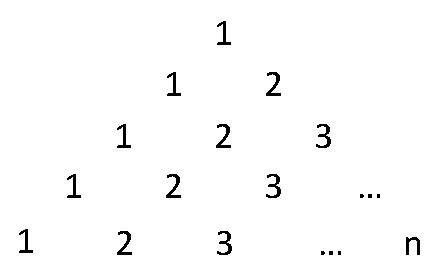
\includegraphics[scale=0.5]{FiguresArithmetic/TetrahedralBasic}
        \caption{Computing $\Theta_n$: basic triangle pattern.}
        \label{fig:TetrahedralBasic}
\end{center}
\end{figure}
and draw two copies by rotating the dimensions.
Fubini's principle is used by summing up the elements in a smart way.

Prove as an intermediate result that the sum of the elements over the rows of the three triangles is proportional to $n+2$.
\medskip

******************}

